%%
%% This is file `sample-sigconf-authordraft.tex',
%% generated with the docstrip utility.
%%
%% The original source files were:
%%
%% samples.dtx  (with options: `all,proceedings,bibtex,authordraft')
%% 
%% IMPORTANT NOTICE:
%% 
%% For the copyright see the source file.
%% 
%% Any modified versions of this file must be renamed
%% with new filenames distinct from sample-sigconf-authordraft.tex.
%% 
%% For distribution of the original source see the terms
%% for copying and modification in the file samples.dtx.
%% 
%% This generated file may be distributed as long as the
%% original source files, as listed above, are part of the
%% same distribution. (The sources need not necessarily be
%% in the same archive or directory.)
%%
%%
%% Commands for TeXCount
%TC:macro \cite [option:text,text]
%TC:macro \citep [option:text,text]
%TC:macro \citet [option:text,text]
%TC:envir table 0 1
%TC:envir table* 0 1
%TC:envir tabular [ignore] word
%TC:envir displaymath 0 word
%TC:envir math 0 word
%TC:envir comment 0 0
%%
%% The first command in your LaTeX source must be the \documentclass
%% command.
%%
%% For submission and review of your manuscript please change the
%% command to \documentclass[manuscript, screen, review]{acmart}.
%%
%% When submitting camera ready or to TAPS, please change the command
%% to \documentclass[sigconf]{acmart} or whichever template is required
%% for your publication.
%%
%%
%\documentclass[sigconf,authordraft]{acmart}
\documentclass[manuscript,review,anonymous]{acmart}
%%
%% \BibTeX command to typeset BibTeX logo in the docs
\AtBeginDocument{%
  \providecommand\BibTeX{{%
    Bib\TeX}}}

%% Rights management information.  This information is sent to you
%% when you complete the rights form.  These commands have SAMPLE
%% values in them; it is your responsibility as an author to replace
%% the commands and values with those provided to you when you
%% complete the rights form.
\setcopyright{acmlicensed}
\copyrightyear{2018}
\acmYear{2018}
\acmDOI{XXXXXXX.XXXXXXX}
%% These commands are for a PROCEEDINGS abstract or paper.
\acmConference[Conference acronym 'XX]{Make sure to enter the correct
  conference title from your rights confirmation emai}{June 03--05,
  2018}{Woodstock, NY}
%%
%%  Uncomment \acmBooktitle if the title of the proceedings is different
%%  from ``Proceedings of ...''!
%%
%%\acmBooktitle{Woodstock '18: ACM Symposium on Neural Gaze Detection,
%%  June 03--05, 2018, Woodstock, NY}
\acmISBN{978-1-4503-XXXX-X/18/06}


%%
%% Submission ID.
%% Use this when submitting an article to a sponsored event. You'll
%% receive a unique submission ID from the organizers
%% of the event, and this ID should be used as the parameter to this command.
%%\acmSubmissionID{123-A56-BU3}

%%
%% For managing citations, it is recommended to use bibliography
%% files in BibTeX format.
%%
%% You can then either use BibTeX with the ACM-Reference-Format style,
%% or BibLaTeX with the acmnumeric or acmauthoryear sytles, that include
%% support for advanced citation of software artefact from the
%% biblatex-software package, also separately available on CTAN.
%%
%% Look at the sample-*-biblatex.tex files for templates showcasing
%% the biblatex styles.
%%

%%
%% The majority of ACM publications use numbered citations and
%% references.  The command \citestyle{authoryear} switches to the
%% "author year" style.
%%
%% If you are preparing content for an event
%% sponsored by ACM SIGGRAPH, you must use the "author year" style of
%% citations and references.
%% Uncommenting
%% the next command will enable that style.
%%\citestyle{acmauthoryear}

\usepackage{CJKutf8}
\usepackage{url}
%\usepackage{hyperref}
%\usepackage{multicol}
\usepackage{multirow}
%\usepackage{array}
%\usepackage{booktabs}
\usepackage[utf8]{inputenc}
\usepackage{balance}
\usepackage{bm}

%%
%% end of the preamble, start of the body of the document source.
\begin{document}
\begin{CJK*}{UTF8}{gbsn}


%%
%% The "title" command has an optional parameter,
%% allowing the author to define a "short title" to be used in page headers.
\title{AI-Driven Design-by-Analogy: A Systematic Review of Representations, Techniques Based on Creative Process and Applications}

%Understanding intelligent creativity from the perspective of Design-by-Analogy: A systematic review of representation, 


%%
%% The "author" command and its associated commands are used to define
%% the authors and their affiliations.
%% Of note is the shared affiliation of the first two authors, and the
%% "authornote" and "authornotemark" commands
%% used to denote shared contribution to the research.


%\author{Lars Th{\o}rv{\"a}ld}
%\affiliation{%
%  \institution{The Th{\o}rv{\"a}ld Group}
%  \city{Hekla}
%  \country{Iceland}}
%\email{larst@affiliation.org}


%%
%% By default, the full list of authors will be used in the page
%% headers. Often, this list is too long, and will overlap
%% other information printed in the page headers. This command allows
%% the author to define a more concise list
%% of authors' names for this purpose.
\renewcommand{\shortauthors}{Trovato et al.}

%%
%% The abstract is a short summary of the work to be presented in the
%% article.
\begin{abstract}

\end{abstract}

%%
%% The code below is generated by the tool at http://dl.acm.org/ccs.cfm.
%% Please copy and paste the code instead of the example below.
%%
\begin{CCSXML}
<ccs2012>
 <concept>
  <concept_id>00000000.0000000.0000000</concept_id>
  <concept_desc>Do Not Use This Code, Generate the Correct Terms for Your Paper</concept_desc>
  <concept_significance>500</concept_significance>
 </concept>
 <concept>
  <concept_id>00000000.00000000.00000000</concept_id>
  <concept_desc>Do Not Use This Code, Generate the Correct Terms for Your Paper</concept_desc>
  <concept_significance>300</concept_significance>
 </concept>
 <concept>
  <concept_id>00000000.00000000.00000000</concept_id>
  <concept_desc>Do Not Use This Code, Generate the Correct Terms for Your Paper</concept_desc>
  <concept_significance>100</concept_significance>
 </concept>
 <concept>
  <concept_id>00000000.00000000.00000000</concept_id>
  <concept_desc>Do Not Use This Code, Generate the Correct Terms for Your Paper</concept_desc>
  <concept_significance>100</concept_significance>
 </concept>
</ccs2012>
\end{CCSXML}

\ccsdesc[500]{Do Not Use This Code~Generate the Correct Terms for Your Paper}
\ccsdesc[300]{Do Not Use This Code~Generate the Correct Terms for Your Paper}
\ccsdesc{Do Not Use This Code~Generate the Correct Terms for Your Paper}
\ccsdesc[100]{Do Not Use This Code~Generate the Correct Terms for Your Paper}

%%
%% Keywords. The author(s) should pick words that accurately describe
%% the work being presented. Separate the keywords with commas.
\keywords{Do, Not, Us, This, Code, Put, the, Correct, Terms, for,
  Your, Paper}
%% A "teaser" image appears between the author and affiliation
%% information and the body of the document, and typically spans the
%% page.
%\begin{teaserfigure}
%  \includegraphics[width=\textwidth]{sampleteaser}
%  \caption{Seattle Mariners at Spring Training, 2010.}
%  \Description{Enjoying the baseball game from the third-base
%  seats. Ichiro Suzuki preparing to bat.}
%  \label{fig:teaser}
%\end{teaserfigure}

%\received{20 February 2007}
%\received[revised]{12 March 2009}
%\received[accepted]{5 June 2009}

%%
%% This command processes the author and affiliation and title
%% information and builds the first part of the formatted document.
\maketitle

\section{introduction}

In the era where foundational models can potentially standardize creativity, amplifying individual output while diminishing collective innovation\cite{doshi2024generative}, understanding, stimulating and applying individual creativity mechanisms is crucial \cite{kawakami2024impact, hitsuwari2023does, humlum2025large} to address this problem. The cognitive science community have extensively studied these mechanisms, encompassing specialized semantic processing\cite{kenett2023semantic}, associative thinking\cite{beaty2023associative}, divergent and convergent thought\cite{mccrae1987creativity}, metaphor and analogy\cite{holyoak1996mental}. In order to explore a pragmatic way of leveraging cognition mechanism in HCI, this work, we focused on Design-by-Analogy(DbA), a goal-oriented field that closely integrates individual cognition with practice, distinguished by its structured mapping nature which enabling qualitative and quantitative measurement\cite{mcadams2002quantitative}, offers a significant pathway for Combinational Creativity\cite{peng2025probing} measurement and stimulate.

%在一个基础模型可能使创造力标准化的时代,放大了个人产出却削弱了集体创新【】,理解、激发和应用个体的创造机制至关重要。认知科学领域对创造性机制的有大量研究,涵盖特殊语义处理【】、联想思维【】、发散/聚合思维【】、隐喻和类比【】等。本文聚焦于类比设计(DbA),这一领域以目标为导向,紧密结合了个体的认知与实践,同时,其结构化映射的本质使该行为能够进行定性和定量测量,为组合创造力提供了一条重要途径。


Design-by-Analogy(DbA) is a design methodology in which novel solutions, opportunities, or designs are generated within a target domain by drawing inspiration extracted from a source domain using specific mapping logic\cite{jiang2022data, fu2014bio, gentner1983structure}. DbA possesses a well-established research foundation within the engineering design field, dating back to the Structure-Mapping Theory in 1983\cite{gentner1983structure}. This initiated a series of computational analogy reasoning studies\cite{hofstadter1984copycat, hummel1997distributed, falkenhainer1989structure, thagard1990analog}. Around 2000, research gradually expanded to focus more explicitly on analogy design, establishing robust frameworks for quantitative assessment and standardized evaluation of DbA processes\cite{mcadams2002quantitative}. By approximately 2010, the emergence of research on wordtree based methods for patent database analysis sparked a renewed surge of interest in DbA\cite{linsey2012design, linsey2008increasing, verhaegen2011identifying}, leading to numerous studies\cite{fu2014bio, fu2015design, jiang2022data}. Researchers explored various methodological aspects of DbA, primarily concentrating on mechanical design\cite{jiang2022data}, bio-inspiration design\cite{fu2014bio} and patent based design\cite{verhaegen2011identifying} contexts. In the wild, DbA applications show the potential: wind turbine blades inspired by humpback whale tubercles by engineers\cite{fu2014bio}, foreign entrepreneurs migrated patents from local perfume manufacturers to innovate alcoholic beverage businesses\cite{andriani2025perfume} and etc.
% %-------类比设计定义,类比设计历史,为何类比设计-------------
%类比设计(DbA)是一种设计方法,通过从源领域汲取灵感,在目标领域中生成新颖的解决方案、机会或设计\cite{jiang2022data, fu2014bio}。DbA在工程设计领域拥有坚实的研究基础,其起源可追溯到1983年的结构映射理论\cite{gentner1983structure}。这引发了一系列关于计算类比推理的研究\cite{hofstadter1984copycat, hummel1997distributed, falkenhainer1989structure, thagard1990analog}。大约在2000年左右,研究逐渐扩展,更加明确地聚焦于类比设计,并为DbA流程建立了可靠的定量评估框架和标准化评价体系\cite{mcadams2002quantitative}。到2010年前后,基于词树的专利数据库分析方法的研究兴起,再次引发了对DbA的浓厚兴趣\cite{linsey2012design, linsey2008increasing, verhaegen2011identifying},进而催生了众多研究\cite{fu2014bio, fu2015design, jiang2022data}。研究人员探索了DbA在方法学方面的各个层面,主要集中在机械设计\cite{jiang2022data}、生物启发设计\cite{fu2014bio}和基于专利的设计\cite{verhaegen2011identifying}等场景。已经投入工业使用的类比设计案例,如:工程设计师受座头鲸鲸鳍上凸起结节的启发设计出了更高效的风力涡轮机叶片, 外来企业家迁移当地专利开展创新业务等。



Although the value of Design-by-Analogy (DbA) has been illustrated through numerous examples, our systematic literature review reveals that current research on DbA in both academia and industry remains fragmented. Existing reviews typically focus on specific perspectives, including DbA theory,\cite{song2018characterizing,linsey2008modality,linsey2008increasing}, data-driven approaches using narrow-scope sources\cite{jiang2022data,fu2014bio,}, applications of single computer technologies\cite{aamodt1994case, chakrabarti2011computer, ghane2024semantic, regenwetter2022deep}, and interaction-centered DbA methods.\cite{tseng2008role, marshall2016analogy, verhaegen2013refinements} Implicit in these works are several assumptions: that DbA is only applicable in the early ideation stage or limited to specific use cases; that it must be supported solely by structured data; and that its representational forms are inherently constrained. Furthermore, we observe a growing trend in the AI industry to compress the creative process into a simplified input–output model. This reductionist view tends to overlook the inherent complexity of design problems\cite{chakrabarty2024art, wadinambiarachchi2024effects} , often resulting in design fixation and considerable resource waste \cite{palani2022don}. In response, this review investigates DbA within a broader design context, with a focus on AI-driven method, examining its diverse representation, analyzing technologies for comprehensive creative processes and their broad applications, highlighting it's cross-modal and cross-domain knowledge integration and computationable potential, asserting its ethical and technology mediation value in activating human innate capabilities\cite{smits2019values, schecter2025role}, and demonstrating industrial applicability to address these research gaps.
% %-------------(1)之前类比设计研究的gap,(2)为什么要基于创作过程拆解,(3)我们怎么填补这些gap-------------------------
%虽然,类比设计的价值通过诸多例证已经展露,但从系统性文献综述的回顾中,我们发现,当前类比设计研究在工业界和学术界呈碎片化态势,不同产业的研究重点关注在创造过程的不同侧面,相关综述包括类比设计理论,单一主题数据源驱动的类比设计,单一计算机技术在类比设计中的应用,以交互方法为中心的类比设计等。这些综述暗含了一些假设,如类比设计的使用场景仅在创意前期阶段或仅支持某些应用场景,类比设计仅能被结构化的数据支撑,以及类比设计的表现形式具有局限。同时,我们关注到创意过程在ai产业界的压缩现象,将创意过程压缩为“输入和输出”的简单过程,而忽略设计问题的复杂性,会导致大量的设计固定及造成资源浪费。因此,本综述在更广泛的设计范畴内研究了基于类比的设计,特别聚焦于人工智能驱动的DbA方法,研究了其多种表现形式,分析了面向全面的创造过程的技术以及其广泛的应用场景,强调其跨模态、跨领域知识整合和计算的的潜力、声明其在激发人类内在能力方面的伦理和技术中介价值,以及其工业适用性,以填补这些研究空白。




Our systematic review of the literature reveals that DbA, as a common cognitive foundation behavior in practice, spans various domains, representing in six forms: \textit{Semantics and Text}, \textit{Visual and Appearance}, \textit{Material and Structure}, \textit{ Function and Attribute}, \textit{Interaction, Workflows, and Multi-sensory experience}, and \textit{Unconventional Contexts}. Supporting four phases of the creative process and their subprocesses, including \textbf{Problem Definition} (vision, inspiration), \textbf{Product Ideation} (ideation, prototype), \textbf{Product Implementation} (fabrication), and \textbf{Product Evaluation} (evaluation, meta). This approach can be applied in creative industries, intelligent manufacturing, education and service industries. For instance, enabling intelligent transfer of similar product principles for new design concepts in creative industries, generating novel mechanical designs and manufacturing processes via data retrieval/mapping in intelligent manufacturing, and facilitating knowledge transfer in education and services industires. Detailed explanations will be provided in Sec.4–6. This study aims to answer three key questions: 
(1) How and why to fully declare the technical mediating value of Deisgn-by-Analogy to help related industries organically utilize and activate practitioners' inner value? 
(2) What is the current state of existing AI-driven DbA technologies? How do they specifically support different human-machine collaboration needs across various stages of the create process?
(3) What general findings and technical guidelines can be provided? Where still require AI support and how?

Findings and responses will be elaborated in Sec.7.
%--------------------------------我们做了什么,我们回答的研究问题-----------------------------
%基于系统性文献综述,我们发现基于类比的设计行为作为各行各业的一种共性的认知基础,横跨在各个领域。其表现形式也多种多样,从语义、外观、结构、功能到流程和特殊语境分为六种形式。基于类比设计的技术可以辅助创意过程的4个大阶段7个子阶段,如问题定义(前景、启发),产品构思(构思、原型),产品操作(制作)和产品评估(评价和元)。该方法可以在创意领域、智能制造、教育和服务业中进行部署。如,在创意工业中基于相似产品原理智能迁移得到新的设计构思,在智能制造领域,根据生物知识检索和映射产出新的机械设计方案及制造工艺规划,在教育和服务业中,通过知识迁移辅助各类教学。我们将在第sec3-6详细解释表现形式、创意过程及应用。同时,本研究尝试回应三方面问题:其一,如何充分阐述类比设计的技术中介价值,以帮助相关行业有机利用并激发从业者的内在价值?其二,现有的AI驱动的类比设计技术的现状如何?在设计过程的不同阶段如何具体支持人机协作的不同需求?其三,有哪些通用的发现和技术指导?还有哪些部分需要以及如何使用AI进行支持?我们将在Sec.7解释我们的发现并回答问题。
The contributions of this work are threefold: 
(1) We conducted a systematic review and PRISMA selection process\cite{page2021prisma} on technologies, applications, and theoretical articles (N = 1615) in Design-by-Analogy and related fields. After screening and inclusion based on a set of criteria, 86 articles were finally included, which will be detailed in Sec. 3.  

(2) Based on the selected articles, two authors independently performed thematic analysis\cite{clarke2014thematic} to establish classification criteria, covering 6 representations, DbA techniques based on 7 creative processes, and 3 application domains. Relevant discussions were conducted to address the second question above.  

(3) Guided by the summary and findings of the corpus, we provide directions for future work to answer the first and third questions.
%-------------------------------------本工作的主要贡献是-------------------------------------
% 本工作的主要贡献是(1)我们对design by analogy及相关领域的技术和应用以及理论文章(n=1615) 进行了系统性综述以及prisma selection流程,并按照一系列标准进行了筛选和纳入,最终纳入了n=86篇文献,将在Sec.3详细描述。(2)根据筛选后的文章两位作者独立进行主题分析,建立分类标准,涵盖6种类比设计的表现形式,面向7个创造过程的类比设计技术,3个应用领域,并进行了相关讨论,以回答上述第二个问题(3)基于对语料库的总结和发现,为未来工作进行指导,回答第一个和第三个问题。

















%---------------------------------------DRAFFFFTTTTTTTTTTTTTTTTTTTTTTTTTTT----------------



% %---------------新的研究机遇是什么---------------
%新的研究基于在于进行更加细致和合理的拆解人类创造行为,这一认知行为已经在各种工业产业中进行部署和应用,只是不同产业关注的创造行为的阶段不同,人机交互领域(hci)的相关开发和研究工作尚未完整拆解各个领域中的共性问题并加以点对点的研究和辅助。在创造行为被压缩成为输入指令-产出这样间断的逻辑链条时,设计固定的问题则很难通过模型的优化和提示词的优化来进行改善,而设计固定发生在创意中的各个阶段【】【【】【】。解构创造行为成为了一种必要性的工作。人类在创造行为中动用的创造力机制中的一个子机制就是类比设计,市面上已有一些相关的工作如【】将草图类比到实际产出,【】将人的共情类比到新的情境中,【】将服务类比到新的市场中。新的研究应该由各个产业的人员关注该产业中的创造过程的全部阶段,完整地激发产业从业人员的创造力,帮助他们找到在行业中应用自己的经验,从而找到自信心和自我价值,而非通过压缩人机交互的过程,而雄辩式的声称可以取代他们的工作。本文的研究问题则是:现有的人工智能驱动的类比设计技术如何在设计过程的不同阶段(例如,灵感激发、构思与原型制作)支持人机协作的不同需求?· 现有的各个领域是怎么使用analogy这个认知机制进行应用设计的?还有哪些部分需要以及将如何用AI进行支持?



% %----------我们做了什么------
%本工作的主要贡献是对(1)这一领域的相关文献从2008年的技术和应用以及理论文章(n=1541)中进行了系统性review,严格执行了prisma selection流程,并按照xxxxxx的标准进行了筛选,排除了1.不服务设计的算法 = 69, 不服务于设计的理论 = 156,不讨论类比设计的文献 = 77,仅验证类比有效性的文献= 91,(2)最终建立分类标准,纳入了n=106篇文献。并进行了总结和讨论,以回答上述问题,(3)我们为未来工作进行指导。

\section{Background}

\subsection{The Cognitive Mechanism of Design-by-Analogy}
%主要写analogy的认知机制,和design by analogy的将认知与实践紧密结合,与创造力的关系,与类比推理的区别,与case based reasoning的区别,以及其可计算的潜力。
Design-by-Analogy (DbA) refers to a design approach in which novel solutions within a target domain are created inspiration from a source domain via cross-domain analogical reasoning.\cite{jiang2022data, fu2014bio} This method centers around a design problem. By procedurally invoking external knowledge, experience, data, and other contents, it aims to stimulate operators' internal experience, memory, inspiration, and motivation. This method is a mechanism where cognition and practice proceed in parallel.\cite{moreno2015step, schecter2025role}.

Analogy, is a cognitive paradigm for the transfer of knowledge between domains\cite{gentner1983structure, hofstadter2001analogy} and it can be actively carried out when individual wants to acquire new knowledge\cite{gentner1997reasoning}. Design, on the other hand, has a strong practical attribute. As an intentional activity that aims to \textit{``transform existing conditions into preferred ones''} \cite{simon2019sciences}, design inherently operates as a goal-oriented practice, requiring physical or virtual implementation to validate conceptual solutions. Thus, Design-by-Analogy constitutes a goal-driven cognitive practice that naturally embeds the cognitive mechanisms of analogy within design processes. 
% 类比设计(DbA)是指一种设计方法,即通过跨领域类比推理从源领域获取灵感,从而在目标领域中创造出新的解决方案。\cite{jiang2022data, fu2014bio} 这个方法是围绕一个设计问题展开的,其通过程序化的调用外部知识、经验、数据等内容,致力于激发操作者的内部经验、记忆、灵感和驱动力。这种方法是一种认知和实践并行的机制。
%类比是一种用于在不同领域之间转移知识的认知范式\cite{gentner1983structure, hofstadter2001analogy},当个体想要获取新知识时,它可以被主动运用\cite{gentner1997reasoning}。另一方面,设计具有很强的实践性。作为一种旨在“将现有条件转变为理想条件”的有目的的活动\cite{simon2019sciences},设计本质上是一种以目标为导向的实践,需要通过物理或虚拟实现来验证概念性解决方案。因此,类比设计构成了一种目标驱动的认知实践,自然地将类比的认知机制融入设计过程中。 
%-------------------------【-DbA介绍-】---------------------

Design-by-Analogy demonstrates several key characteristics. First, the DbA process integrates the analogy-making process\cite{french2002computational} and the computation-able mechanisms\cite{gentner2011computational}, structured into four stages: representation/ encoding, retrieval, mapping and evaluation\cite{jiang2022data, fu2014bio, fu2015design}. Second, DbA usually has an \textit{``open goal''}\cite{tseng2008role} and typically combines intrinsic and extrinsic triggers\cite{moreno2015step, moreno2016overcoming}, enabling the human brain to link stimuli with memory concepts for the generation of ideas\cite{goucher2019neuroimaging}. Third, empirical and neuroinformatic evidence shows \cite{moreno2015step, goucher2019neuroimaging} that DbA can assist designers in overcoming design fixation through stimulation and analogical exploration.
%类比设计具有一系列特点,首先,类比设计过程综合了类比制作及计算机制,分为四个阶段表征/编码,检索,映射,评估四个阶段,通过相似特征的结构化映射将检索到的源域内容转换为目标域内容。其次,类比设计通常拥有一个开放性目标,结合内部刺激和外部刺激方法,使人脑将刺激与记忆概念连接,生成新想法。第三,类比设计被实证\cite{}和神经信息\cite{}手段证明可通过刺激和类比探索来辅助设计师突破设计固定。
%------------------------------【-DbA的特点-】--------------------


This practice-oriented nature enables DbA to directly harness analogical reasoning\cite{gentner1983structure, gentner2011computational, linsey2008increasing} for creativity support through three core mechanisms: First, DbA embeds the structured cognitive mechanisms\cite{french2002computational} into the creative process to scaffold the analogical reasoning of individuals in different stages of creative work\cite{hsueh2024counts}. Secondly, human goals and internal values will guide the direction of DbA divergence. In DbA, analogy is not aimless, but is constrained by human factors such as design goals, design factors, design problems, and the internal values of designers\cite{moreno2015step, chan2011benefits}.
Third, DbA internalizes the creativity computation. Due to the common analogical structure as \textbf{`` A:A'=B:B' ''}\cite{gentner1983structure}. The explicit cognitive operations in this process allow for algorithmic implementation and automated deployment, Methods such as symbolic models\cite{falkenhainer1989structure}, connectionist model\cite{thagard1990analog, hummel1997distributed} and hybrid models\cite{hofstadter1984copycat}, has been applied in many industrial scenarios. DbA organically integrates human cognition, creative behavior, and computer automation via the above three aspects, supporting creative computability without compromising human will.
%这种以实践为导向的特性使设计行为分析能够直接利用类比推理——检索和映射源 - 目标关系——通过三种核心机制来支持创造力:
% 首先,DbA 将类比构建的结构化认知机制(识别、细化、迁移、巩固\cite{french2002computational})融入创作过程,以支持个人在不同创作阶段的类比推理。【类比设计的基本认知实践相结合的能力】
% 其次,人的目标和内在价值会指导类比设计的发散方向, 在这之中,类比不是漫无目的,而是受设计目标,设计因素,设计问题,设计师的内在因素等人因约束。【类比设计的人因本质】
% 第三,类比设计将创造力计算内化。这一过程中的显式认知操作允许算法实现,例如符号模型\cite{falkenhainer1989structure}、联结主义模型\cite{thagard1990analog, hummel1997distributed}和混合模型\cite{hofstadter1984copycat},并且已经进行工业应用。【类比设计可自动化】
%类比设计通过以上三点将人的认知、人的创造行为、计算机自动化有机融合,支持创造力可计算的同时,不会丢弃人的意志。
%---------------【DbA激发创造力的机制】-------------------------


Unlike other creativity supporting methods, Design-by-Analogy have several advantages. In converting novelty to practicality, DbA outperforms than unstructured brainstorming\cite{linsey2010study}. When prioritizing the activation of human creativity, DbA reduces cognitive load compared to pure analogical reasoning\cite{richland2013reducing}. When compared with Case-Based Reasoning (CBR) method, for it's automated paradigm in retrieve-reuse-refine-restore, DbA involves a higher degree of human factors and creativity remaining\cite{wills1994towards} which can facilitate more on human intrinsic value stimulating.

% 与其他支持创造力的方法不同,在将新颖性转化为实用性方面,类比设计优于无结构的头脑风暴\cite{linsey2010study}。在考虑激发人类创造力方面,与纯粹的类比推理相比,这种综合方法降低了认知负荷\cite{richland2013reducing}。与基于案例的推理(CBR)相比,由于CBR在检索 - 重用 - 改进 - 恢复方面采用自动化范式,而DbA涉及更高程度的人为因素和创造力\cite{wills1994towards}。
%-------------------【-DbA和其它方法的对比-】---------------------------------









\subsection{Related Survey}

The concept of Design-by-Analogy develops after the birth of the structure mapping theory in 1983\cite{gentner1983structure}. Between 1983 and 2010, substantial foundational work emerged in this field, including evaluation metrics\cite{mcadams2002quantitative} and computational models\cite{french2002computational, gentner2011computational, falkenhainer1989structure, thagard1990analog, hummel1997distributed, hofstadter1984copycat}. Around 2008, after Linsey et al. introduced the WordTree method to Design-by-Analogy\cite{linsey2008increasing}, a series of studies applying this method to mechanical design\cite{fu2015design}, biological analogical design\cite{fu2014bio}, conceptual design\cite{moreno2016overcoming}, etc.


Today, DbA widely used in various fields of human activities. In biomimetic industry, classic cases in the wild include scientists inventing radar based on bat echolocation\cite{fu2014bio}. In academic, researchers have proposed function-behavior-structure design frameworks\cite{helms2009biologically}, related taxonomies\cite{fu2014bio}, and challenges\cite{nagel2018establishing, linsey2013overcoming}. In mechanical design, engineers developed more efficient wind turbine blades inspired by humpback whale fin tubercles which is already widely deployed in real world\cite{linsey2008increasing}. Studies in mechanical design field, focus on constructing patent migration databases\cite{fu2015design} and methods to prevent design fixation\cite{atilola2015representing, marshall2016analogy}. In product design, designers have drawn analogies from dump trucks to create cat litter boxes\cite{linsey2012design} and research efforts on analogy migration methods\cite{barnett2002and}, specific techniques\cite{ghane2024semantic,liu2023smfm, regenwetter2022deep, ghane2024semantic,}, design synthesis\cite{chakrabarti2011computer}, and interactive systems embedding cognitive mechanisms\cite{goel2012cognitive}. In education, scholars explored the analogy methods in education design\cite{duit1991role}. In philosophy and mathematics, DbA is studied as design metacognition\cite{ball2019advancing, holyoak1996mental} and a mathematical problem-solving and situation awareness approach\cite{polya2020mathematics}.

%%1983年结构映射理论诞生后,基于案例的类比推理随之发展起来\cite{gentner1983structure},在1983-2010年间,本领域有许多基础工作诞生,如相关的评价标准,计算模型等。在2008年前后,由linsey等人将wordtree方法引入类比设计领域后,一系列使用此方法的工作专注专利数据,生物数据,众包创意等应用层出不穷。至今,基于类比的设计行为广泛存在人类活动的各个领域中。在仿生工业领域,仿生设计中的代表案例是科学家依据蝙蝠的回声定位原理发明雷达,研究人员提出了功能-行为-结构的设计框架【】以及相关的分类法【】和挑战【】;机械设计中,工程师根据座头鲸的鲸鳍结节发明更高效的风力涡轮机叶片,研究人员专注于构建专利迁移数据库【】以及预防设计固定的方法【】【】;产品设计中,有设计师根据自卸卡车设计猫砂盆的先例,研究人员致力于研究各类方法,各类数据库,产品本体的类比迁移以及内嵌认知机制的交互研究【】【】【】;在教育行业中,研究人员使用类比设计【】【】【】研究教科书的源域近域等等;在哲学和数学领域,也有研究纯粹的类比作为设计元认知的,类比作为数学解题和情境感知法的内容【】【】
%--------------------------【-类比设计的历史和在各个领域中的应用及survey-】----------------


%我们对调研的相关调查分类并指出了相关的研究gap
We classified the relevant surveys and pointed out the research gaps. Surveys focusing on data include Jiang et al.'s study on data-driven analogical design theory \cite{jiang2022data}. Linsey et al.'s research on data representation and modality\cite{linsey2008modality}, and efficiency in DbA\cite{linsey2010study}. Barnett et al.'s focus on knowledge representation and transfer in analogy \cite{barnett2002and}. Fu et al. and Nagel et al.'s investigation into taxonomies of analogical design across different data types and themes \cite{fu2014bio, nagel2018establishing}. What’s more, O'Rourke et al.'s work on using BID data to address energy efficiency in mechanical design \cite{o2015toward}.
Surveys on algorithms and techniques include Chakrabarti et al.'s review of computer-based design synthesis \cite{chakrabarti2011computer}. Ghane et al.'s exploration of semantic Theory of Inventive Problem Solving (TRIZ) techniques in design \cite{ghane2024semantic}. Regenwetter et al.'s focus on deep generative models for engineering design \cite{regenwetter2022deep}. Dimassi et al. focused on the application of knowledge recommendation in 4D printing \cite{dimassi2023knowledge}. Liu et al.'s development of an analogical retrieval tool for innovative product concept design based on the structure-mapping function model (SMFM), proposing eight mapping types \cite{liu2023smfm}. Moreover, Aamodt et al.'s case-based reasoning (CBR), which has informed numerous computational models and techniques and shares similarities with DbA \cite{aamodt1994case}. Khanolkar et al.\cite{khanolkar2023mapping} mapped 7 AI methods to 5 design processes.
Surveys on interaction and evaluation include Tseng et al.'s study on the impact of analogical design provision timing \cite{tseng2008role}. Marshall and Atilola's research on analogy representation, proposing mechanisms affecting design fixation and creative processes \cite{atilola2015representing, marshall2016analogy}. Goel et al.'s exploration of cognitive science-empowered computer-aided design systems \cite{goel2012cognitive}. Verhaegen et al.'s review of existing idea evaluation metrics \cite{verhaegen2013refinements}. Lu et al.'s analysis of analogical design impacts across different stages \cite{lu2023differences}. In addition, Song et al.'s investigation into how different analogical information influences participants \cite{song2018characterizing}.
%专注于数据的survey包括Jiang等人专注数据驱动的类比设计理论\cite{jiang2022data},lindsey等人研究类比设计过程中数据的呈现,模态及效率【】【】,barnett等人关注类比中知识数据的表征和迁移\cite{barnett2002and},fu等人研究不同的数据和不同主题的类比设计分类法\cite{vio,patent},O等人则关注使用BID数据解决机械设计中的能源效率问题\cite{o2015toward},
%专注于算法和技术的文章有:Chakrabarti等人调研了基于计算机的设计合成\cite{chakrabarti2011computer},ghane等人探索了设计过程中使用语义Theory of Inventive Problem Solving(TRIZ)技术的可行性\cite{ghane2024semantic},Regenwetter等人专注深度生成模型如何应用于工程设计\cite{regenwetter2022deep},Dimassi 等人关注知识推荐在4d打印中的应用\cite{dimassi2023knowledge}。此外,liu等人基于structure-mapping function model (SMFM) 调查了创新产品概念设计类比检索工具并提出了八种映射类型\cite{liu2023smfm}。Aamodt等人提出的casebased reasoning(CBR)支撑了许多计算模型和技术的产生,与类比设计有异曲同工之妙\cite{aamodt1994case}, Khanolkar等人将7种ai方法映射在5个设计流程中。
%专注于交互和评估的survey包括Tseng等人关注不同时机提供类比设计的影响\cite{tseng},marshall和atilola等人关注类比表示研究,提出了影响设计固着和创造过程的不同方式\cite{atilola2015representing, marshall2016analogy},Goel等人探索了基于认知科学赋能的计算机辅助设计系统\cite{goel2012cognitive}, verhaegen等人调查了现有的想法评估指标\cite{verhaegen2013refinements},lu等人调查了不同阶段使用类比的不同影响\cite{lu2023differences},song等人调查了不同类比信息对参与者的影响\cite{song2018characterizing}

%--------------------------【-类比设计在数据、算法和技术、交互和评估三个方面的survey】----------------





Research gaps remain in the literature on DbA surveys: Firstly, existing reviews predominantly focus on specific disciplines or technical approaches, treating DbA as a tool serving fragmented domains, rather than considering disciplines and technical means from a panoramic perspective with human creativity itself as both the starting point and the objective. While a related survey\cite{jiang2022data} addresses mechanical design and data-driven approaches, it overlooks ambiguous data and applications beyond its scope. Researchs map the semantic TRIZ and AI techniques into creative stages but neglects designers' creativity supportive\cite{khanolkar2023mapping, ghane2024semantic}. Secondly, current work concentrates on single data sources or implicitly assumes DbA supports only on text, ``function-behavior-structure'' ontology and visual, ignoring other representations. Thirdly, disparate taxonomy persist across disciplines, lacking a unified framework centered on the creative process. This paper establishes a systematic review from the perspective of computational creativity, positioning human creative behavior as the core subject. By investigating the representation of DbA, summarizing techniques based on the creative process, and examining its application domains, we explore how DbA can augment individual experience-based creativity, bridge epistemological gaps, and reinforce human subjective value in the AI era.
%当前关于类比设计的调查有一些尚且没有被填补的空白:首先,当前综述多聚焦特定学科(如机械、生物、增材制造)或技术手段(如NLP-TRIZ、CV、3D打印),将类比视为服务分散领域的工具,而非以人类创意本身为出发点和目标全景式地考虑学科及技术手段。相近研究【】局限于机械设计与数据驱动,忽略模糊数据及其他领域应用,【】【】将技术方法映射在创造阶段中,但是忽略了设计师的创造力因素;其次,现有工作关注单一数据源(如专利数据、仿生学、岩土制造),或默认类比设计仅支持文字、功能或形态等模态数据,未考虑类比设计的其他表现形式;再者,各学科存在割裂的分类体系,缺乏创造过程视角为中心的统一分类框架。本文以计算创造力为研究视角,以人的创造行为为主体,建立系统性综述,通过调研类比设计的表现形式,总结基于创造过程的类比设计技术以及类比设计的应用领域,探索类比设计如何辅助个体基于经验的创造力,弥合认知论断层,在AI时代强化人的主体性价值。

%--------------------------------【目前研究gap】




























%-------------------draft---------------

%2. (1)目前没有根据设计创意阶段解构的类比设计survey,大多数survey关注的是用于模拟认知方法开发的技术、将类比设计应用于某一具体设计内容的,如机械,产品,生物,增材制造(AM)等,他们关注的视角本身就不是创造这件事情本身为中心,而是类比这种方法怎么服务于特定的分散的学科,与我们调研scope最相近的是这篇【】但是他的关注重点在机械设计和数据驱动,忽略了模糊数据和除机械设计以外的类比设计。(2)还有许多survey讲的是某一具体技术怎么进行类比的辅助,如nlp-triz技术,cv技术,3d打印技术怎么辅助类比这个工作而已,他们的聚焦中心是某一特定的技术领域,多类比设计中非该技术手段可以辅助的部分他们便不考虑了,也就是说他们不考虑类比设计的最终结果,而是考虑他们的技术能做哪一部分的类比,哪一个侧面的类比。(3)聚焦于某一特定数据来源/模态,比如patent data(专利数据),bio mimicry,岩土制造,机械,图形数据库等,单一文字或者单一图片的survey模态,他们考虑的是单一来源的数据,关注点是如何利用某一大型数据集来辅助特定的类比项目。
%【我们关注类比辅助的创意过程本身,是一个whole picture的survey,探索如何用这种方式更好的辅助人的创造行为】

%3.目前类比存在多元分类,在不同学科领域呈现出差异化的分类形式,尚未有统一的创意过程视角下的分类。在哲学领域,依据《哲学词典》的分类体系,类比可分为质料类比、形式类比、综合类比、对称类比、因果类比与协变类比六种形式。质料类比基于事物间的物质属性相似性进行分类,如将不同金属的导电性类比;形式类比则侧重于事物结构或关系的相似性等。这些分类主要依据类比所涉及的属性类型与关系特征进行划分。而在数学领域,类比主要包括降维类比、升维类比、结构类比等。在认知科学领域也是单独的定义类比,在机械设计中相关的survey也有许多,包括也有许多理论和技术在分布似的散点一样的在各大研究领域中展开,他们都为本工作提供了重大灵感支撑。【这一部分没人做过】

%% 4. 其他survey没有将类比设计当作一种创造力机制作为基础而将其他领域知识当作垂类知识库来进行系统review,没有将人的创造行为抬升到某一前所未有的高度,这一工作可以弥合许多领域的认知论gap,我们希望人关注到个体的认知行为的背后原因是希望人在ai时代通过有意识地觉察自己的思考逻辑和期待的事情发展方向,建立自己的主体性,关注人本身的特质,以及我们的愿景是希望individual可以通过计算到达的多元的发散的多彩的,而非统一的单一价值取向的目的地,探索一条新的渠道,释放不同个体的基于经验和个性化特征的创造力。本survey辅助的则是这一过程,不拘泥于任何强调非人创造行为以外的学科、技术、技巧、社会议题等干扰项。



















\section{Literature review Methodology} %zs
This chapter aims to systematically review and analyze the current research status of the field of \textbf{AI-driven DbA}. To ensure the comprehensiveness and rigor of the literature collection process, this study followed the PRISMA guidelines\cite{page2021prisma} for systematic review and conducted a multi-stage iterative evaluation and inclusion process. As illustrate in Fig.\ref{fig:prisma-selection}

\subsection{Data Collection}
\textbf{Identification Stage}:
In the identification stage, this study initially obtained several pieces of literature in applications and technologies of design by analogy (N = 990), AI-driven analogy (N = 104), theory and taxonomy of creative processes (N = 24) through a combination of manual and programmatic retrieval in fields such as human-computer interaction, computer science, design studies, cognitive science, mechanical design and bio-design. After initially identifying a set of literatures, 17 core seed literatures with high citation rates in their respective retrieval fields and high alignment with the direction of this study were identified from the above initial literatures. Subsequently, we conducted forward( N = 30)and backward( N = 30) snowballing on each of themobtaining a total of 658 literature pieces in this process after duplicate removing. In total, 1,615 literatures were collected. The retrieval keywords or phrases used in the corpus construction included ``\textit{Design-by-analogy}'', ``\textit{Analogy Reasoning}'', ``\textit{Analogical Design}'', ``\textit{Case-based Reasoning}'', ``\textit{Analogy Making}''. After deduplication, 1,378 pieces remained. 
\subsection{PRISMA Selection}
\textbf{Screening Stage}:
In the Screening stage, this study ensured the precision of the corpus through multiple filtering processes. First, we used a programmatic approach to quickly identify and eliminate literature that was clearly unrelated to the topic based on titles and abstracts. Subsequently, two researchers independently read and manually screened ambiguous literature. In this stage, we eliminated \textbf{EC1}: literature pieces with duplicate titles ($N = 237$), \textbf{EC2}: those without peer review ($N = 23$), and \textbf{EC3}: irrelevant pieces ($N = 545$), leaving 682 articles in the corpus.

\textbf{Eligibility Assessment Stage}:
In the eligibility assessment stage, two researchers applied a series of explicit exclusion criteria to screen and assess the full text content of potential literature, ensuring the quality of the final corpus. Specifically, we removed: \textbf{EC4}: literature where analogy was merely used as a computational intermediate method with the objective of pure algorithmic analogy research (N = 69); \textbf{EC5}: literature that did not directly serve creative work and processes\cite{hsueh2024counts} (N = 156); \textbf{EC6}: literature that used analogy as an ideational method in domain-specific research but did not delve into its connotation (N = 177); \textbf{EC7}: literature that only validated the effectiveness of DbA and other related empirical studies (N = 91); \textbf{EC8}: literature that did not use broad-spectrum artificial intelligence to drive DbA but relied on other computational methods (N = 59). After this stage, 130 articles remained in the corpus.

\textbf{Inclusion Stage}:
To ensure the thematic relevance and classification coverage of our corpus, the corpus covers all relevant categories, including theory, application, and technology, we strive to ensure an even distribution of literature under each major category. Two author independently using thematic analysis\cite{terry2017thematic} and iterative discussions on the previously screened literature and conduct the taxonomy system, further eliminated 20 pieces that did not meet the research criteria or thematic repetition. A total of 106 literature pieces were retained.
Through the above process and iteration between stages, this study ultimately constructed a highly relevant and representative corpus for the field of AI-driven DbA, with a total of 86 literature pieces included for subsequent literature analysis and review.


\begin{figure}
    \centering
    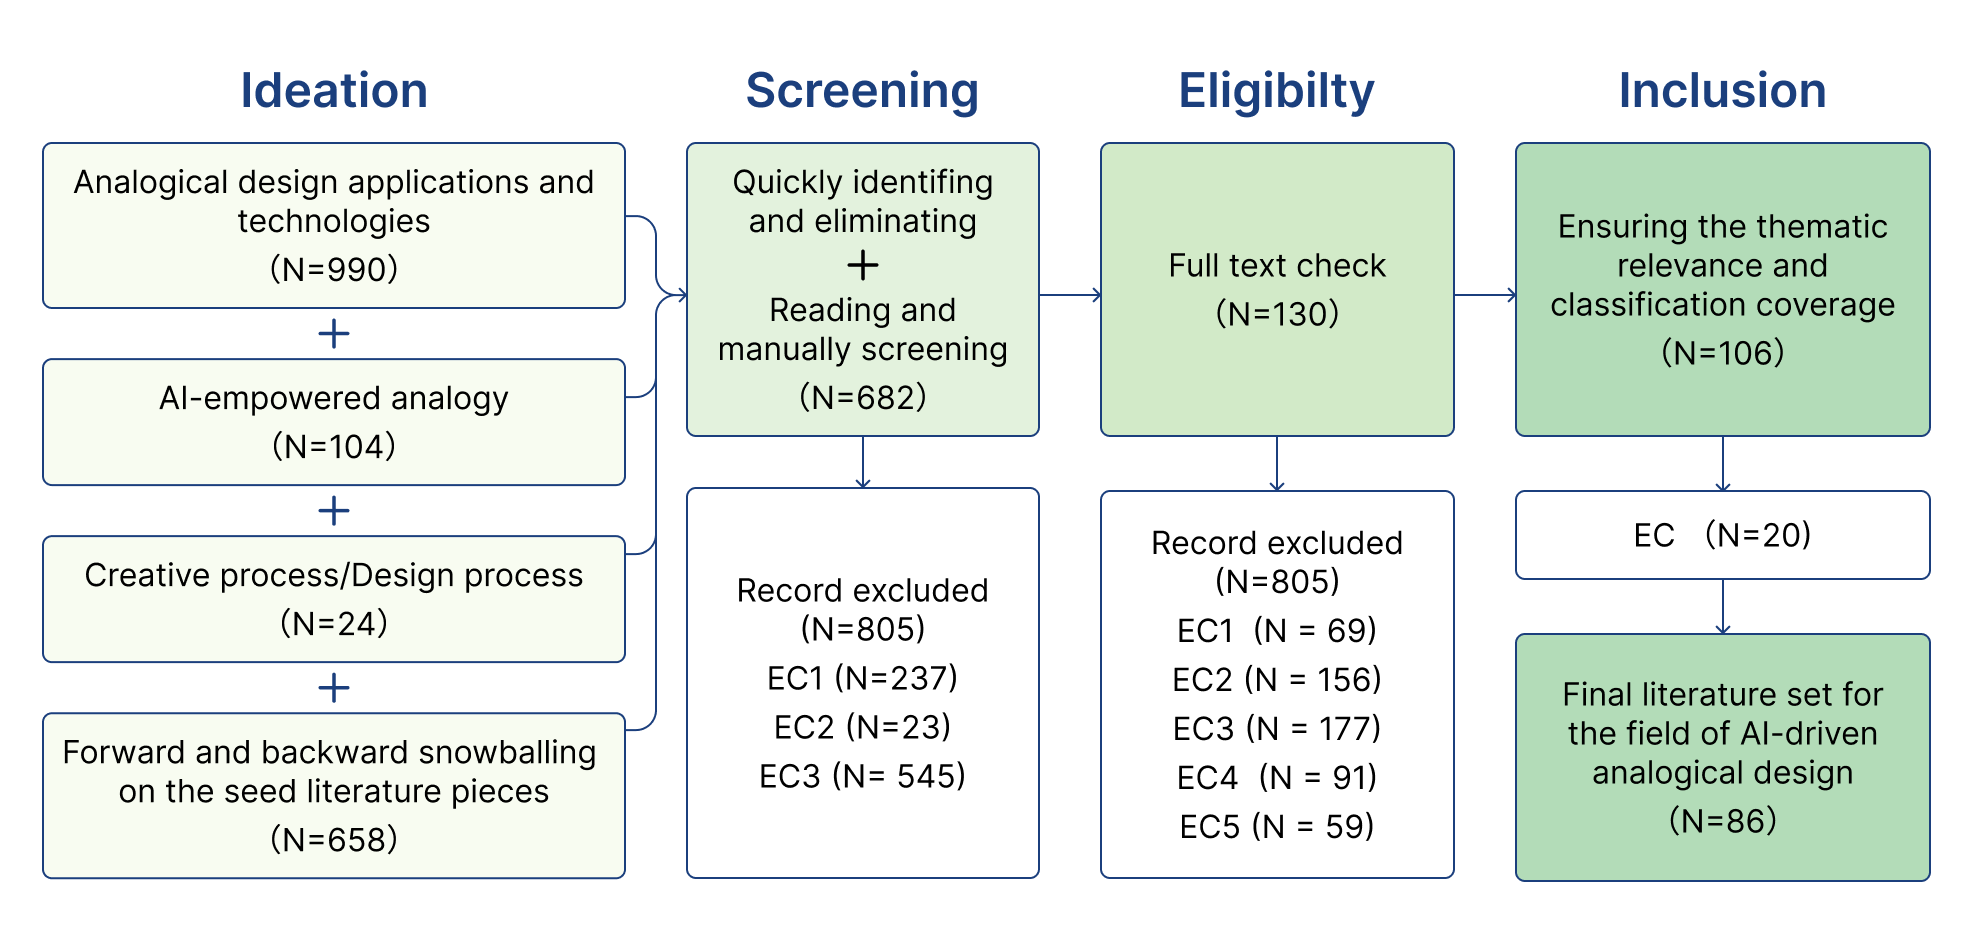
\includegraphics[width=1\linewidth]{Figures/prisma selection.png}
    \caption{This figure presents a literature screening process that adheres to the PRISMA guidelines, detailing the step - by - step filtering of publications across four phases: Collection, Screening, Eligibility, and Inclusion. Explicit exclusion criteria (EC1–EC5, such as duplicate titles, irrelevance, and the absence of peer review) and the changes in the number of publications at each stage are shown. It clarifies how the initial large literature pool (N = 1,816) is gradually refined into a final set of 20 publications that meet the requirements of thematic relevance and methodological rigor.}
    \label{fig:prisma-selection}
\end{figure}



%prisma
%相关关键词可以加一些引用,这是前两段内容,第三节也可以逐步写一下

% %本章节旨在系统性地回顾和分析\textbf{AI驱动的类比设计}领域的现有研究现状。为确保文献收集过程的全面性和严谨性,本研究参考系统评价报告指南PRISMA流程进行多阶段迭代评估及纳入。具体而言,文献筛选过程主要分为识别阶段、筛选阶段、资格评估阶段和最终纳入阶段。

% 识别阶段:
% 在识别阶段,本研究首先通过手动收集和程序化检索相结合的方法,在人机交互、计算机、设计学、认知科学、机械设计、生物设计等领域初步获得了类比设计相关应用及技术文献990篇、人工智能赋能的类比相关文献104篇、创意过程/设计流程相关文献24篇。同时,在初步识别一系列文献后,我们从上述初始文献中,识别出17篇在各自检索领域内引用率较高且与本研究方向高度契合的核心种子文献(如图?所示),随后对这些种子文献进行了程序化的前向和后向滚雪球,各30篇,此过程共获得文献658篇。共计1,615篇,去重后1378篇,检索中使用的核心关键词或词组包括Design-by-analogy、Analogy Reasoning、Analogical Design、Case-based Reasoning、Analogy Making,文献检索的时间范围设定在1983年至2025年。
 
% 筛选阶段:
% 在筛选阶段,本研究通过多重过滤筛选确保文献库的精准性。首先,我们使用程序化方式根据标题和摘要快速识别并剔除与主题明显不相关的文献。随后,2名研究人员对一些模糊文献进行逐一独立阅读和人工筛选。此阶段剔除了标题重复的文献237篇、未经同行评审的文献23篇、无关文献545篇,文献池剩余文章682篇。 

% 资格评估阶段:
% 在资格评估阶段,2名研究人员应用了一系列明确的排除标准对潜在文献进行了逐篇全文内容筛查及评估,从而保障最终文献库的质量。具体而言,我们剔除了移除了:EC1 类比仅作为计算中间环节,用户无法感知到的纯粹算法类比研究(N = 69);EC2 文献不直接服务于创造过程, 参考hsueh et al.提出的创造工作定义\cite{hsueh2024counts}的文章(N = 156);EC3 文献在研究方法中使用类比这一方法但未深入探讨其内涵的文献(N = 177);EC4 文献仅验证类比设计有效性及其他相关实证研究的文章(N=91),EC5 应用文献没有使用广义的人工智能进行类比设计驱动而是用其他方式(N = 59)此阶段文献池剩余文章130篇。 

% 最终纳入阶段:
% 为了确保最终文献库在主题相关性与分类覆盖度上差异分布,文献库需尽可能涵盖所有相关的分类,包括理论、应用和技术,并力求保证每个主要分类下文献分布均匀,共保留文献106篇。在建立分类法后,我们对前期筛选出的文献进行了主题审阅和讨论,并进一步剔除了20个不符合研究标准的文献。   
% 通过上述系统性、多阶段的文献收集和筛选过程,本研究最终构建了一个与AI驱动的类比设计领域高度相关且具有代表性的文献集合,最终纳入了86篇文献用于后续的文献分析和综述。 
\subsection{Corpus Overview}
%本研究通过系统性的多阶段筛选流程,构建了一个包含86篇文献的语料库,这些文献在主题相关性、分类覆盖度和研究质量上具有高度代表性。语料库涵盖了从1983年至2025年的研究成果,反映了AI驱动的类比设计领域在不同时期的发展趋势。文献分布均衡地覆盖了理论研究、应用实践和技术方法等多个主要分类,为深入地分析该领域提供了坚实基础。


%可能有一张barchart图
\section{Representations in Design-by-Analogy} %数字是飞书-论文筛选-论文归类sheet1的序号
We refer to previous work\cite{hertzmann2023image, linsey2008modality}, articles related to the analogy theory\cite{gentner1983structure}, and the corpus collection, we obtain the following forms of representation.
%我们参考以往工作和analogy理论相关文章基于语料库收集得到如下表现形式。

%语义/文字
\textbf{\underline{Semantics and text.}} It refers to make analogy at the concepts and contextual semantic levels. This can be stratified into several tiers: The first level is using textual analogies for identifying similarity, leveraging narrative analogies in personalized writing and crowdsourced creative writing ideation. For instance, Shao et al. and Ju
et al. employ analogy generation at the sentence/phrase level to produce empathetic stories and comprehensible scientific instructional content \cite{shao2025unlock, Ju2025toward}. Srinivasan et al. and Yu et al. utilize crowdsourced ideation, chunking, and recombination to generate novel far-domain analogical inspirations or innovative design concepts\cite{srinivasan2024improving, yu2014distributed}. The second level is using lingustic concepts as the domain transfer mediation, for instance, Researchers respectively achieve cross-disciplinary, cross-manufacturing-process, and cross-modal conceptual mapping through retrieval of relevant knowledge\cite{zheng2024disciplink, emerson2024anther, chen2024BIDTrain, yan2023xcreation} . And works compile domain knowledge into text-centric repositories for function tracking and context mapping in geotechnical engineering, service design, data products, and military systems \cite{you2018design, moreno2014analogies, chen2024beyond, yucelmics2018procedure}.

%语义和文字的定义是在概念和上下文语义上进行类比。分为几个层次,第一个层次是使用文字类比来识别相似性,在个性化写作和众包创意写作构思中利用叙事类比。如【49】【44】工作利用类比法生成语句字段级别的类比,产出令人产生同理心的故事和令人理解的科学教学内容;【1】【5】工作使用众包创意、组块和重组等方法生成新的远域类比灵感或者新的设计概念和构思。第二个层次是使用语言概念作为领域转移的中介,例如,【13】【3】【7】【15】分别是通过检索相关的知识,完成跨学科的,跨制造工艺,跨模态的概念映射;【72】【76】【10】【60】将领域知识总结为文字为主的知识库用于岩土工程、服务设计、数据产品、军事产品的功能追踪、情境映射等。


%仅外观/形状
\textbf{\underline{Visual and Appearance.}} It refers to make visual analogies of lines, colors, style, etc. at the appearance level. 
The fundamental type is elementary visual similarity for aesthetic forms, where works such as Warner et al. employ geometric shape correspondences to achieve vector graphic style transfer\cite{warner2023interactive}, Lin et al. investigate sketch migration\cite{lin2025inkspire}, and Fischer et al.'s 3D model based analogies\cite{fischer2024nerf}. There are still some tasks based on visual concepts generalization, with \cite{yu2016distributed, edwards2024advise} dedicated to mining and generating design concepts grounded in visual resemblance. The second type is visual context relationship mapping, where Akula et al. focuses on interpreting and generating visual metaphors through semantic relations among pictorial elements\cite{akula2023metaclue}, whereas Bitton et al. addresses context-aware visual scene understanding and synthesis\cite{bitton2023vasr}. The third type is cross-domain structural remapping, as implemented in Gong et al.'s work remaps faces from creatures/films to specific faces via structured mapping\cite{gong2023toontalker}, while Peyre et al. detects and generates visual relational similarities (e.g., actions, semantics, behaviors) overlooked by conventional approaches\cite{peyre2019detecting}.

%在外观层面进行线条、色彩、风格等视觉上的类比,分为几个层次:第一个层次是使用视觉元素的相似性类比生成艺术设计作品,如【9】【50】【20】工作通过几何形状相似性生成矢量图形的样式迁移,草图的迁移以及模型相似性上的类比,还有一些工作【36】【35】致力于挖掘或生成基于视觉相似性的设计概念上的类比;【25】关注画面元素之间的语义关系,进行视觉隐喻的映射的理解与生成,而【18】工作关注并致力于理解和生成基于情境感知的视觉画面;而【27】这份工作基于结构化映射将人脸从别的生物和影片中跨域重演到特定人脸上,【26】工作致力于检测并生成传统方法忽略了的动作、语义、行为上的视觉关系相似性图片。



%材质/结构
%在材料、结构上进行类比
\textbf{\underline{Material and Structure}}. It refers to make analogical mapping at the material physical properties and structural levels. Here we categorized as follows: First, works achieve cross-domain migration through the similarities of physical properties such as material, finishing, strength, thermal conductivity, ductility, etc. For example, in product design, Fischer et al. and Khosravani
et al.'s work perform material and finishing migration according to the knowledge bases\cite{fischer2024nerf, khosravani2022intelligent}. Thomas et al. mapped mechanical fatigue characteristics to the visualizations of the factory monitoring systems\cite{thomas2013extending}. Hong et al. converting biological tissue elastic modulus to wearable flexible electronics\cite{hong2024fishbone}. Moreover, An et al. mapped the manufacturing process of wooden frame components and the experience of automated manufacturing onto new frame throught Computer Numerical Control(CNC) Machine Tool\cite{an2020bim}.
Secondly, microstructural analogy based on geometric topology (lattice, porosity, fiber arrangement): Fan et al. leverage fractal design analogies with stretchable electronic structures\cite{fan2014fractal}. Jin et al. using buckling-guided Assembly principles mapping 2D patterns to 3D structures\cite{jin2023deep}. Yu et al. investigate structural mapping of cephalopod chromatophore mechanisms to triple-layer color-changing materials\cite{yu2014adaptive}.

% %在材料物理属性与结构层面进行类比。 分为以下层级:
% 通过物理属性,如材质、工艺、强度、导热性、延展性等相似性实现跨领域迁移,如在产品设计时根据知识库进行材质和工艺迁移【20,67】,将机械疲劳特性映射到工厂检测系统的可视化上【77】,在柔性电子领域的将生物组织弹性模量转化为柔性电子器件的可穿戴设计【64】,【78】将木框架组件的制造工艺及自动化制造经验映射到新制品上;cnc加工
%基于微观构造,如晶格、孔隙、纤维排布的几何拓扑类比,如分形设计与可拉伸电子结构的类比【30】,依据屈曲组装原理的抽象结构类比2d图案与三维框架结构【86】,将头足类动物的三层细胞变色特性结构化映射到三层变色表皮材料【65】




%功能/属性
\textbf{\underline{Function and Attribute.}} It refers to make analogical mapping at the levels of same problem solving mechanisms, working principles, and relational isomorphism. Here we categorized as follows level: First, functional consistency analogy, leveraging core functional similarity where the same function solves the same problem, exemplified by Murphy et al's retrieval functions through database\cite{murphy2014function}. Zhang et al recommending new software features based on product data analysis\cite{zhang2017systematic}, and Khosravani et al. mapping built-in knowledge bases to new contexts for solutions \cite{khosravani2022intelligent}. Secondly, distinct-principle analogy, applying knowledge of different principles from other domains to solve the same problem, such as Kang et al. transferring mechanical function knowledge from biological knowledge bases \cite{kang2025biospark}, Gonzalez et al. optimizing energy supply using behavioral knowledge from building spaces \cite{gonzalez2018energy}, and Kittur et al. investigate scaling knowledge for innovation via AI and crowdsourced ideas \cite{kittur2019scaling}. Third, analogy based on relational niches and structural equivalence, demonstrated by chen et al. using text/images proportional to complex data relationships for communication \cite{chen2024beyond}, Karunathilaka et al. explaining quantum concepts via analogy in AR \cite{karunathilaka2025intuit}, and Emerson et al. retrieving/mapping craft tutorials based on similarity in material practices \cite{emerson2024anther}.
%在解决问题的相同性上进行类比,工作原理,关系和属性上的相似性
% 【%功能/属性
% 在问题解决机制、工作原理及关系同构性层面进行跨域类比映射。 分为以下层级:利用核心功能一致性进行类比,同一功能解决同一问题:搜索功能的类比设计方法\cite{murphy2014function},基于产品现状进行数据分析并推荐软件新功能\cite{zhang2017systematic},基于内置知识库映射到新的情境中提供解决方法\cite{khosravani2022intelligent}
% 通过其他领域的不同原理的知识,解决同一问题:基于生物知识库中寻找机械功能实现知识迁移\cite{kang2025biospark},通过检测并记录建筑空间内的人的行为形成经验知识优化能源供给\cite{gonzalez2018energy}, 通过结合ai和众包创意扩大知识规模从而促进创新\cite{kittur2019scaling}
% 关系生态位上的相似性,结构等效性上进行映射:使用与复杂数据内容比例和关系一致的文案/图像进行内容传达\cite{chen2024beyond},通过ar场景下的类比解释量子计算概念\cite{karunathilaka2025intuit}, 通过操作材料的具体实践的相似性进行手工教程检索及映射\cite{emerson2024anther}





%交互/流程/多模态
\textbf{\underline{Interaction, workflows, and multi-sensory experience.}} It refers to operate analogies across interaction modalities, workflows, and multisensory integration. This encompasses: First, interaction similarity, exemplified by \textit{Textoshop} mapping graphic software interactions to text-editing design\cite{masson2025textoshop}, and \textit{Umitation} transferring interaction methods between websites using target cases\cite{chen2021umitation}. Secondly, there are similarities in transactional workflows such as design, operation, execution, and evaluation. Demonstrated by Lauff et al. mapping additive manufacturing processes to modular ontologies for operational enhancement \cite{hagedorn2018knowledge}, Riguard et al. capturing overlooked execution data in manufacturing workshops for future knowledge reuse \cite{rigaud2022exploring}, Lupiani et al. generating future care decisions through temporal reasoning of elderly home behaviors \cite{lupiani2017monitoring},Coley et al. applying robotically reconfigurable workflow apparatus achieve organic compounds automatic synthesis\cite{coley2019robotic}. Third, based on the mutual mapping and transfer between sensory experiences and multimodal content. Illustrated by \textit{STAR }transferring physical typing sensations to AR for enhanced experiences \cite{kim2023star}, Reelframer translating news texts into narrative videos \cite{wang2024reelframer}, and \textit{Drone Chi} mapping Tai Chi movements to human-drone interaction behaviors \cite{la2020designing}.
%在交互方式、工作流程和跨模态,多感官结合层面的类比
%在交互上具有相似性,如Textoshop将绘图软件的交互式操作映射到文本编辑软件的设计上【4】,Umitation通过目标网站交互案例实现源网页交互方法映射\cite{chen2021umitation]。
%在设计、操作、执行、评估等事务性流程上具有相似性,Lauff et al.【56】将增材制造的流程映射到新的模块化本体上增强操作,【59】Riguard et al.捕捉制造工作坊中易被忽略的执行数据并在未来作为知识经验使用,lupiani等人通过时态案例和老年人居家行为推理和生成未来养护决策【85】caley等人将可机器人操作的化合物合成流程自动化,结合预测算法实现自动化化合物合成
%基于感官感受和多模态内容之间的互相映射和迁移,STAR【8】将现实中的打字行为和感受迁移到增强现实中以增强体验,reelframer【15】将源新闻文本映射为叙事视频,Drone chi【75】将太极动作和行为映射到人与无人机交互的行为和体验上。





%非传统语境
\textbf{\underline{Unconventional Contexts.}} This refers to abstract analogies based on cultural trends, niche knowledge, or unique experiences rely on specific expertise and local cultural contexts. These analogies embody highly original and personalized connotations. For example: La et al.embedded Tai Chi culture into \textit{Drone Chi} emerging technologies\cite{la2020designing}. Andriani et al. transformed local resources through adaptive modification based on local knowledge systems and analogical search mechanisms, converting perfume manufacturing processes into winemaking techniques\cite{andriani2025perfume}. Cao et al. compiled domain-specific interdisciplinary terminology into \textit{MedAI-SciTS} to support personalized analogy lexicons to facilitate cross-disciplinary collaboration\cite{cao2025medai}. Christensen et al. leveraged heterogeneous team members' background knowledge to mutually stimulate analogies during collaborative design\cite{christensen2016creative}.
%基于文化潮流、小众知识、特殊经历的抽象类比,仰赖设计师内在经验、在地文化等特殊内容的类比,具有非常原创性以及个性化的内涵。比如,Drone chi【75】将太极文化嵌入到新兴技术中,【66】等人基于在地知识文化和类比搜索机制对本地资源束进行适应性改造,将香水制造工艺转为制酒工艺,【39】MedAI-SciTS将特性领域之间的跨学科术语总结成个性化类比词表以供跨学科协作,【69】异构背景的设计团队协作相互调用背景知识激发类比



\begin{figure}
    \centering
    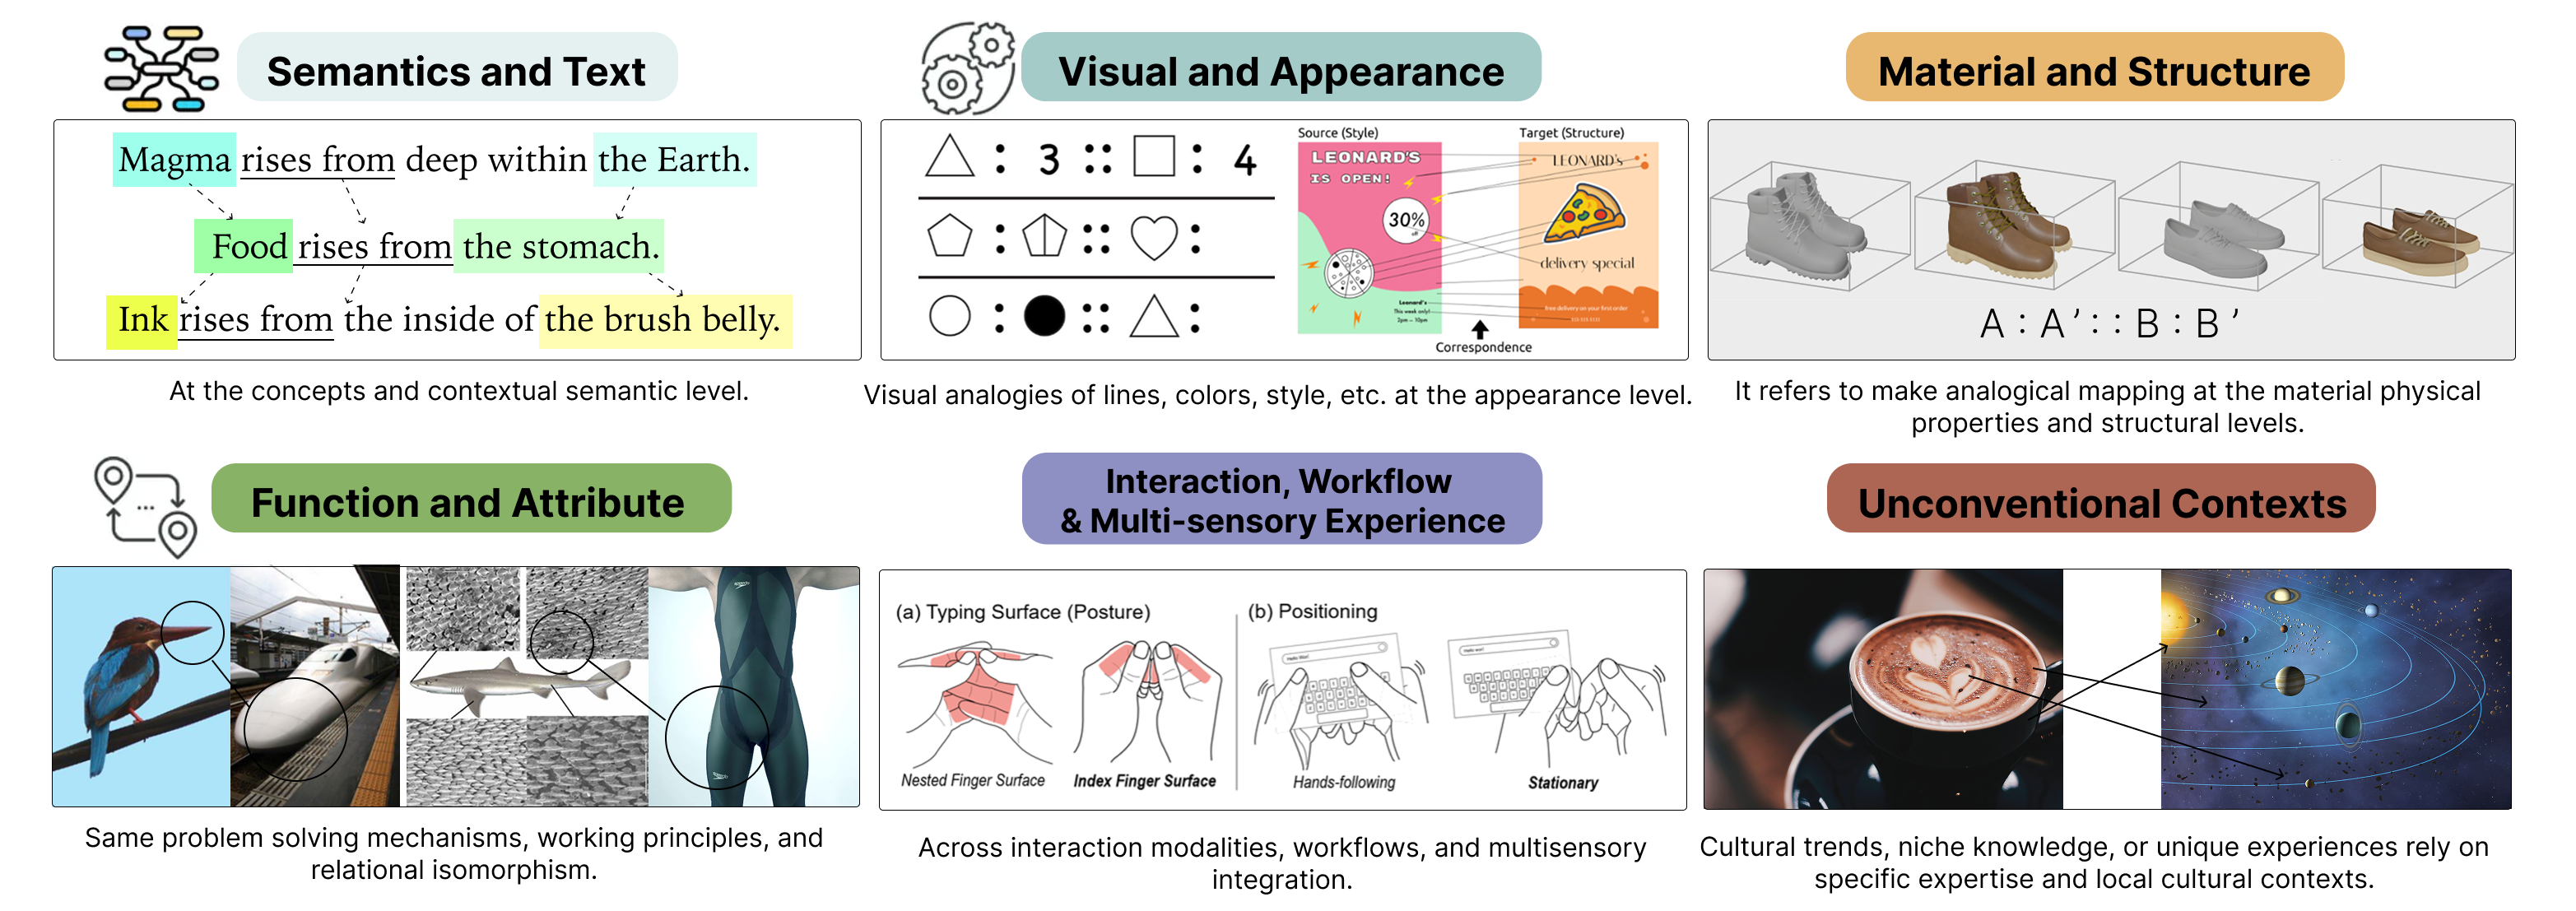
\includegraphics[width=1\linewidth]{Figures/representation.png}
    \caption{Enter Caption}
    \label{fig:Representation}
\end{figure}
\section{DbA Techniques Based on Creative Process}
We refer to previous work and articles related to the creative process definition\cite{frich2019mapping, chung2021intersection, hsueh2024counts, cross2021engineering, keates2002user, weaver2010transformation} to collect the techniques based on the creative process and provide corresponding cases based on corpus collection. It is worth mentioning that most of the work does not only serve one stage. The division is based on the maturity of ideas, the entire process is categorized into 4 primary stages and 7 iterative sub-processes, to emphasize the forms and contents that DbA technique can assist. At each stage, we will classify cases into three levels: Assist, Augment, and Automate, based on the degree of human-computer collaboration, and describe them accordingly. At the Assist level, the software assists with specific techniques such as screening, retrieval, and mapping to reduce cognitive load. At the Augment level, human-computer collaboration stimulates thinking and creativity. At the Automate level, the machine iterates on content independently, with humans assisting in the iteration direction.
%我们参考以往工作和creative process理论相关文章得到基于创造过程的技术分类,并基于语料库收集给出一些相应的案例。值得一提的是多数工作并不仅服务于一个阶段,加以划分只是强调类比设计可以辅助的形式和内容。在每个阶段,我们将根据人机协作的程度,将案例分为三个层级进行描述,分别是:assist、augment和automate。在assist层级软件辅助筛选、检索、映射等相关具体技术,减轻认知负荷,在augment层级人机协作相互刺激思考和创造力,automate则是机器自主迭代内容,人辅助迭代方向。

%Assist (人机筛选结合) < Augment (Co-create人机相互刺激) < Automate (机器自主迭代) 90%
\subsection{Phase 1: Problem Definition}
The core mission of this phase is to precisely define problems by revealing structural contradictions rather than initiating a design based on superficial statements\cite{simon2019sciences, hsueh2024counts} as illustrate in Fig \ref{fig:Create Process}. Defining the design problem confronts three dilemmas: (1) Arbitrary starting points risk solution-target misalignment and resource waste. (2) When existing solutions fail to resolve issue. For example, in 1996, the Brazilian policy was hindered by the lack of basic data and interface design\cite{barzelay2007learning}, it is necessary to identify the real pain points. This process relies on interdisciplinary experience, and those without experience are difficult to be competent. At this time, DbA can assist in attribution and the transfer of indirect experience. (3) Entrenched traditional methods often compel visionary designers to compromise with classical cases\cite{wills1994towards}. We use the metaphor of standing under the wall and cannot see the landscape outside the wall to represent the dilemma in \textit{Vision} phase and standing on the information and experience provided by DbA system will get into the \textit{Inspiration} phase in Fig.\ref{fig:Create Process}. Integrating DbA assists in problem definition can through content tracing and inference while expanding conceptual horizons\cite{hewstone1990ultimate}, assisting designers to internalize visions and missions, providing the possibility to solve the problem mentioned above. The technological content processed at this stage is diverse, fragmented, distributed across domains, and governed by ambiguous logic\cite{li2010agentsinternational}.
%此阶段创造任务的核心在于精准定义问题本质、揭示结构性矛盾,而非基于表面陈述直接设计。定义设计问题面临三重困境:首先,武断的起点易导致方案偏离目标并引发资源浪费;其次,当既有方案无法解决问题时(如1996年巴西政策因基础数据与交互设计缺失受阻),需识别真实痛点,该过程依赖数据采集与界面设计经验,无经验者难以胜任,此时类比设计可辅助归因与间接经验传递;最后,传统方法的根深蒂固常迫使前瞻性设计师妥协于经典案例。引入类比设计,能通过深度溯源与因果推断准确定义问题,同时提供开阔思路,帮助设计师内化愿景和任务,为解决上述困境提供可能。此阶段的技术所处理的内容是多元碎片化的、跨领域分布的、模糊逻辑的。

\textbf{\underline{Vision.}} Technology at this stage aims to provide artistic inspiration and visionary support for those with vague problems, such as market and user research, risk prediction and etc. At the \textit{Assist} level, within the decision-making contexts of software feature development, Zhang et al. employs DbA theory based recommendation techniques for similar product features to conduct user research and infer development directions\cite{zhang2017systematic}. Similarly, He et al. utilize multi-modal technologies to mine and characterize existing case libraries for assisted directional ideation for future transportation system design\cite{he2019mining}. At the \textit{Augment} level, during preliminary market observation and decision formulation in international investment, Li et al. propose a multi-agent integrated decision support application that leverages knowledge bases, simulations, and fuzzy logic to enhance investment direction forecasting\cite{li2010agentsinternational}. Concurrently, in creative design, researches have shown that collaborators with different cognitive depths in problem articulation can inspire participants and AI robots to construct multiple visions for the same problem\cite{yu2014distributed, chan2014conceptual, christensen2016creative}. At the \textit{Automate }level, scenarios applied DbA methods to generate heuristic direction, such as using topic modeling firm management assessment for policy strategy\cite{gavetti2005strategy}, defining specific problem for service design\cite{moreno2014analogies}.
%此阶段的技术旨在为那些面临模糊问题(如市场/用户调研、风险预测等)的人提供艺术灵感和前瞻性支持。 在辅助(Assist)层级,软件功能开发决策的研究中,文献 【19】采用基于设计知识库(DbA)理论的相似产品功能推荐技术执行用户调研并推导开发方向;类似地,文献 【68】通过多模态技术挖掘与表征案例库以支持定向交通系统规划构思。在增强(Augment)层级,国际投资理财领域的前期决策阶段,文献 【84】开发了集成多智能体的决策辅助应用,结合知识库、模拟推演及模糊逻辑提升投资方向预判能力;创意设计领域的研究 【5,33,69】则表明,不同认知深度的合作者阐述问题可激发参与者/机器对同一问题的多元愿景建构。在自动化(Automate)层级,诸如使用主题建模的企业管理评估【79】、服务设计问题定义【76】等场景有很多工作已应用DbA方法来生成启发式方向。


\textbf{\underline{Inspiration.}} It refers to the assistance in inspiration stimuli and design heuristics through DbA techniques. Research at this stage demonstrates diversified technical approaches. At the \textit{Assist} level, Zhu et al. extract bioTRIZ inspired innovation stimuli through functional case modeling of biological functions\cite{zhu2023design}. Emuna et al. use semantic retrieval and reasoning models to build a search engine for mining biological-analogical design inspiration from websites\cite{emuna2024imitation}. Murphy et al. employ the vector approach and hybrid model to search for inspiration\cite{murphy2014function}, and Moreno et al. utilize the rule-based case library for the retrieve and generate of solutions\cite{moreno2014fundamental}. \textit{AskNatureNet} further facilitates the divergent thinking to stimulate inspiration through structured knowledge visualization\cite{chen2024asknaturenet}. At the \textit{Augment} level, \textit{AnalogiLead} enables linguistic chunk and recombination via interaction design for perceiving more analogy ideas\cite{srinivasan2024improving}, and Kang et al. integrate several resource platforms to trigger inspiration through visual and text stimuli\cite{kang2025biospark}. \textit{AnalogyMate} confirms textual prompts stimulate proportional data reflection\cite{chen2024beyond}, whereas \textit{BIDTrainer} enhances knowledge acquisition via structured interfaces\cite{chen2024BIDTrain}. At the \textit{Automate} level, \textit{STORYANALOGY} leverages large language models to mine and generate narrative-level creative analogies\cite{jiayang2023storyanalogy}, Warner et al. use the interactive flexible method to achieve direct cross-domain style transfer\cite{warner2023interactive}, and \textit{VASR} method accomplish context-aware analogical image recognition and synthesis\cite{bitton2023vasr}.
%指的是通过DbA技术在灵感激发和设计启发方面提供的帮助。该阶段研究呈现多维技术路径分化:在辅助(Assist)层级,Zhu等人 [57]基于功能案例建模从生物效应角度提取BioTRIZ创新启发,等人使用语义搜索和推理模型构建了从网络挖掘生物类比设计灵感搜索引擎[24],Murphy等 [53]采用混合模型搜索类比灵感,Fu等人 [40]运用规则驱动的案例库检索生成方案,而AskNatureNet [38]则通过仿生知识可视化引导发散思维;在增强(Augment)层级,研究 [1]利用交互设计实现类比组块重组,文献 [2]借助资源网站推荐系统触发生物类比联想,[10]证实文字提示可激发数据比例反思,BIDTrainer [7]则通过结构化界面促进新知吸收;在自动化(Automate)层级,STORYANALOGY [16]依托大语言模型挖掘叙事级创意类比,方法 [9]实现跨领域风格映射的直接生成,VASR等系统则完成情境化类比图像的识别与合成,



\subsection{Phase 2: Product Ideation}

The core objective of this phase is to derive a feasible design solution based on the prior definition of the problem and exploratory analysis. As the ideation phase commits around 80\% of the project costs, its quality of decision-making critically determines the performance of the sustainability of the product\cite{kerzner2025project}. Research indicates that Design-by-Analogy (DbA) systems effectively mitigate resource waste and overcome design fixation through each stage of it's procedure\cite{o2015toward}. By integrating domain knowledge data\cite{jiang2022data} and experience repositories, this approach automates the abstraction of source problem and the generation of the target solution, producing innovations characterized by convergence, goal-oriented, and deep integration of user needs\cite{fu2015design}. During transition between the sub-process, such as from ideation to prototype, DbA can assist structural refinement of a certain framework, aesthetic enhancement of the overall appearance and scheme polishing of the transactional work.
%本阶段的核心任务是根据前期的问题定义和相关探索得出一个可行的设计方案。设计构思阶段作为锁定80%项目成本的核心环节,其决策质量直接影响商品可持续性表现\cite{kerzner2025project}。研究表明,基于智能类比设计(Design-by-Analogy, DbA)的系统可通过编码-检索-映射-评估机制,结合领域知识库与模糊经验库实现源域问题抽象化及目标域方案生成,有效规避资源浪费并突破设计固定效应。该方法产出方案兼具收敛性、目标聚焦性及用户深层需求融合性。在从构思过渡到原型的过程中,基于类比设计(DbA)可辅助结构优化、美学提升和方案完善。事务性工作


\textbf{\underline{Ideation.}} Distinct from inspiration, this phase involves design convergence, where DbA technology assists users in synthesizing multiple inspirations into ideas. At the \textit{Assist} level: Kim et al. employ Bayesian case-based modeling for prototype generation\cite{kim2014bayesian}. Han et al. develop generative computational tools using 16 ontologies with image and knowledge databases\cite{han2018computational}. Bitton et al. construct visual analogy datasets through situation recognition annotation and CLIP models\cite{bitton2023vasr}. He et al. achieve directed design convergence through conceptual space mining\cite{he2019mining}. Luo et al. stimulate design ideation by regulating knowledge distance\cite{luo2021guiding}. Chen et al. assist ideation leverage semantic-visual combinatorial models\cite{chen2019artificial}and other techniques\cite{akula2023metaclue, you2018design, shen2022nature}. At the \textit{Augment} level: \textit{Pedagogical Prism} implements domain isomorphic analogies\cite{bettin2023pedagogical}. \textit{EmoSync} enables personalized empathy using affective reasoning\cite{Ju2025toward}. \textit{BioSpark} provides interactive analogy suggestions to help the idea mature\cite{kang2025biospark}. \textit{VISION} facilitates inspiration generation and integration through patent visualization\cite{song2020exploration}. At the \textit{Automate} level: Zhai et al. leverage case-based methods autonomously mapping executes irrigation scheduling in viticulture\cite{zhai2020applying}. Caley et al. applied a retrosynthesis prediction algorithm and robotic workflow to automate the synthesis of organic compounds\cite{coley2019robotic}. Moreover, Zhang et al. implemented the autonomous decision making module for intelligent process planning for digital twin manufacturing cells (DTMC) based on deep learning\cite{zhang2020deep}.
%区别于inspiration,这一阶段包含思维的收敛,指的是通过DbA技术辅助用户将众多灵感收敛成为一个新的idea。
%在辅助(Assist)层级,kim等人使用贝叶斯案例模型基于案例和原型进行生成【6】,han等人开发了基于16种本体和图像、知识数据库进行类比推理的生成式计算工具【45】,Bitton等人使用情景识别注释和CLIP模型构建了大规模候选类比数据集用于识别和生成情境类比【18】,He等人【68】通过概念空间挖掘与表征实现定向创意构思,Luo等人通过调整知识距离引导数据表证从而激发设计思考【41】,chen等人通过语义构思网络和视觉概念组合模型辅助构思【54】,其他种类技术【25,72,47】
%在增强(Augment)层级,Pedagogical Prism将领域同构类比作为计算机教育中的启发【48】,基于微侵犯情境,ju等人使用情感推理和内容生成辅助个性化共情【49】,BioSpark通过生成和交互辅助用户完成类比构思并给出建议【2】,VISION 则通过可视化专利知识库促进灵感交互生成【71】
%在自动化(Automate)层级,【12】葡萄种植中的灌溉调度,在基于学习机制的机器上根据案例检索和当前状态自主完成映射,inkspire通过类比草图迁移辅助设计概念探索和完善【50】,【80】使用基于案例的自动规划有机化合物流动合成平台,【81】zhang等人基于深度学习实现数字孪生制造单元(DMTC)的智能工艺规划.


\textbf{\underline{Prototype.}} This phase involves DbA technology that assists users in refining, upgrading, and iterating predefined ideas. At the \textit{Assist} level: \textit{Textoshop} adopts image editing logic for textual Boolean operations\cite{masson2025textoshop}. Dimassi et al. recommend multimaterial knowledge through semantic similarity vectors to  faclitate intelligent 4D printing\cite{dimassi2023knowledge}. In addition, Liu et al. employ SMFM-based tools enable similar product details retrieval for prototypes\cite{liu2023smfm}. At the \textit{Augment} level: \textit{Umitaton} extracts and edits user-interface(UI) response behaviors for front-end development projects\cite{chen2021umitation}. \textit{InnoGPS} visualizes patent databases for innovation recommendations\cite{luo2019computer}. Moreover, \textit{Xcreation} generates narrative illustration prototypes through cross-modal generation\cite{yan2023xcreation}. At the \textit{Automate} level: Fischer et al. accomplish autonomous 3D attributes analogical transfer  leverage NeRF method\cite{fischer2024nerf}. Zhang et al. achieve 2D visual analogy transfer using CNN and hierarchical GCN\cite{jin2022visual}. \textit{Toontalker} implements facial animation re-targeting with Transformer architectures\cite{gong2023toontalker}.
%这一阶段指的是dba技术帮助用户围绕一个预设好的idea进行打磨,升级和迭代。
%在辅助(Assist)层级,Textoshop利用图片编辑的逻辑迭代文字编辑,如对文本片段进行布尔运算以构建更复杂的文本【4】,Dimassi等人基于语义相似性向量空间为多材料4d打印推荐知识【63】,基于smfm的产品检索推荐工具【61】,
%在增强(Augment)层级,【32】umitation提取、编辑目标网站的ui行为并将其应用于设计项目,【62】InnoGPS开发基于云的专利库可视化检索工具为专利推荐创新,Xcreation基于图文跨模态生成叙事插画原型【15】
%在自动化(Automate)层级,fischer等人基于神经辐射场nerf迁移示例3d模型的属性【20】,zhang等人基于卷积神经网络(CNN)和层次结构的图卷积网络(HGCN)将学习到的视觉知识实现视觉类比迁移和生成【74】,toontalker基于transformer实现人脸动画的重演原型【27】



\subsection{Phase 3: Product Implementation} 
This phase focuses on the implementation of a certain idea with its finalized basic logic, tangible output, and standardized production. Although DbA methodologies are predominantly applied to early-stage creative research and it's efficiency is obvious, a few work focus on the implementation of fabrication phase of DbA. This phenomenon reveals an epistemological gap between the implementation of DbA methods in practical operational techniques: The practical operational experience with strong discreteness and case specificity is difficult to be transformed into structured knowledge\cite{rigaud2022exploring}. This gap lead to the neglects of relevant experiential and embodiment data: replicable techniques\cite{schulz2014design}, niche manufacturing practices\cite{scopigno2017digital}, and embodied cultural knowledge\cite{vaisey2009motivation} face erosion without quantitative documentation. Consequently, the transfer of manufacturing experience based on DbA remains underexplored. We argue that DbA has significant potential here: In intelligent manufacturing, as long as automated production lines leverage computable material processing, where DbA-based cross-domain mapping can balance fabrication creativity and accuracy through controllable structural transfers\cite{schulz2014design}. As for cultural preservation, niche craftsmanship requires digitization through standardized parameters, transforming tacit knowledge into living repositories, where DbA can play the essence technique role for preserving and enlivenment through it's unique technology mediation nature\cite{scopigno2017digital, jiang2022data}.
%本阶段创意任务的核心是围绕具体方案实施操作、产出落地及标准化生产。类比设计领域普遍将类比设计方法用于创造前期研究,同时,制造研究者普遍关注具体的实操阶段的技术,这中间存在认知论gap,即,强离散性与案例特异性的实践操作经验难以转化为结构化知识。这一认知导致相关经验数据被忽视——可复现工艺技术、小众制造实践与具身化文化知识因缺乏量化记录而面临消亡。因此,DbA驱动的制造业经验传递成为研究洼地。我们认为DbA在此具有巨大潜力:智能制造中,只要自动化产线依赖可计算材料处理,那么基于DbA的跨领域映射就可以通过可控结构迁移平衡制造创造力与准确性。至于文化保护,小众工艺需要通过标准化参数实现数字化,将隐性知识转化为活态知识库,在这方面,基于数据的类比(DbA)可以凭借其独特的技术中介性质,发挥关键技术作用,实现文化的保护与传承\cite{scopigno2017digital, jiang2022data}。 


\textbf{\underline{Fabrication.}}
This phase covers manufacturing, development, production, and deployment, where DbA technologies enhance user implementation. At the \textit{Assist} level, You et al.'s geotechnical decision supporting system with embedded craft data\cite{you2018design}can help making detailed implementation decision. Jin et al. leverage deep learning assisted buckling-guided assembly design for 3D frame structures producing\cite{jin2023deep}, and other mentioned manufacturing assistance techniques\cite{hong2024fishbone, dimassi2023knowledge, yu2014adaptive} share the same logic. The \textit{Augment} level, \textit{Anther} applies cross-domain video tutorial retrieval for transfer of niche craftsmanship techniques
\cite{emerson2024anther}. In addition, Schulz et la. develope a system which can design,assembly and manufacturing 3d products making using example data base \cite{schulz2014design}. Riguad et al. 's robotic system are able to collect craft data automatically in niche workshops for experience recommendation\cite{rigaud2022exploring}, and Khosravani et al. deploy knowledge-based DbA methods for injection molding lines in the intelligent processing machine\cite{khosravani2022intelligent}. At the \textit{Automate} level, Zhai et al.'s case based reasoning system for agricultural irrigation can be embeded in smart city and grid infrastructures\cite{zhai2020applying}. Moreover, An et al.'s BIM-based automated manufacturability checking for wood frames\cite{an2020bim}, and automated decision support systems\cite{gonzalez2018energy, zhang2020deep, lupiani2017monitoring}are categorized in our work as facilitating fabrication phase.
%这一阶段则包含了实际的制造、开发、制作、部署等,该阶段的dba技术可以增强用户的实施操作。
%在辅助(Assist)层级,You等人基于内置制造技艺数据的岩土工程决策支持系统【72】,基于深度学习辅助三维框架结构力学组装设计【86】,相似的前文提到过的【56】【63】【65】也涉及到制造辅助
%在增强(Augment)层级,anther实现基于跨领域同制作工艺和概念的视频制造教程检索【3】,基于可制造产品数据库进行组装,拼接,设计和制造【52】,rigaud等人在小众制造工坊中部署自动化采集制造技艺技术并致力于未来经验推荐【59】,在智能制造的注塑工艺生产线中加入基于知识库的dba方法辅助【67】。
%在自动化(Automate)层级,zhai等人开发了可在智慧城市和智能电网中内嵌的农业灌溉类比推理系统【12】,基于建筑信息模型(BIM)的木框架组件可自动化制造性检查决策支持系统【78】,以及前文提到过的【82,81,85,】


\subsection{Phase 4: Product Evaluation} This phase focuses on monitoring and evaluating the life cycle of a product performance, leveraging different metrics, user feedback, risks, market response, projected outcome, and relevant policies to enable optimization, prevention, alerting, communication, and maintenance for a better product\cite{moreno2014fundamental}. Many products lack production evaluation and analysis over life cycle, resulting in many aspects being considered and implemented only after deployment.\cite{zhong2017intelligent}. DbA techniques can facilitate concurrent sustainability evaluation of product during development through data-driven case analysis and fuzzy logic assessment, enhancing holistic product sustainability\cite{liao2021priming}.
%这一阶段,创意工作的主要目标是检测和评估产品的全链路上的各项性能指标、用户反馈、风险、市场反响、预期结果、涉及到的政策等加以优化、预防、警示、传达、维修等。很多产品缺少全链路的生产评估和分析,导致许多内容是在全面部署后才开始思考和执行. 类比设计可以在开发阶段同时根据数据、案例、模糊逻辑评估设计,促进产品可持续发展。

\textbf{\underline{Evaluation.}} This phase enables DbA technologies to evaluate, predict and provide critiques, feedback and suggestions on previously completed designs. At the \textit{Assist} level, Arditi et al. predict the result of construction litigation using case data \cite{dougan2022predicting}, \textit{CAM} employs evaluation functions to assess the quality of creative analogy\cite{bhavya2023cam}, Boteanu et al. interpret analogy meanings and questions through semantic networks\cite{boteanu2015solving}, and Hill et al. evaluate analogy making precision through contrasting abstract relational structures\cite{hill2019learning}. At the \textit{Augment} level, \textit{BioSpark} automatically generates solution recommendations and feedback for an idea\cite{kang2025biospark}, \textit{Anther} computes conceptual distance and ``concept gravity'' scores to evaluate analogies similarity between different  niche fabrication \cite{emerson2024anther}. Moreover, Malone et al. forecast the distribution of profit and equity in supply networks through contest network design \cite{malone2017putting}. At the \textit{Automate} level, Thomas et al. extend and automate the optimization and generation of maintenance requirementss for software and mechanical systems using system theoretic hazards analysis (STHA)\cite{thomas2013extending}, An et al. conduct automated manufacturability checks\cite{an2020bim} , with similar approaches applied in\cite{coley2019robotic, zhang2020deep, gonzalez2018energy}.
%这一阶段的dba技术可以评估,预测,建议,反馈前期已经完成的设计。
%在辅助(Assist)层级,基于案例数据预测建筑工程诉讼结果【14】,cam使用评估函数评估创意类比的质量【16】,使用语义网络解释类比问题【23】,通过对比抽象关系结构评估类比制作【29】。
%在增强(Augment)层级,Biospark系统自动提供方案的建议和反馈【2】,anther通过计算评估概念距离和concept gravity score来评估类比【3】,通过竞赛网络设计实现根据供应网络的利润和股权分配的预估【34】
%在自动化(Automate)层级,
%【77】Thomas等人基于系统理论危害分析,扩展和自动化软件和机械的优化、维修等需求的生成与分析,【78】an等人进行自动化可制造性检查,相似的还有【80,81,82】

\textbf{\underline{Meta.}}
This phase enables DbA technologies to facilitate global management of design processes. At the \textit{Assist} level, Andriani et al. argue that using mapping method can facilitate end-to-end perfume production workflows transfer to global practices in wine-making provide an example for automation the supply chain migration\cite{andriani2025perfume}, similar examples as shown in\cite{you2018design, song2020exploration}. At the \textit{Augment} level, Cao et al.'s analogy tool support interdisciplinary collaboration between AI researchers and medical specialists for their overall communication and terminology translation\cite{cao2025medai}, while \textit{Analogies to Succeed} employs global transactional workflows mapping and transfer to support service design management\cite{moreno2014analogies}, similar example\cite{karunathilaka2025intuit, wills1994towards, bettin2023pedagogical, li2010agentsinternational}. At the \textit{Automate} level, Thomas et al. extract future iteration requirements for a product across both software and mechanical development processes data set to support global design practices\cite{thomas2013extending}, similar example\cite{yu2016distributed, bitton2023vasr, lupiani2017monitoring}.
%这一阶段的dba技术致力于全局管理整个设计。%在辅助(Assist)层级,将香水生产的全链路映射到酿酒制造产业的全局实践【66】供应链迁移
%在增强(Augment)层级,类比工具辅助人工智能研究员和医学专家之间的跨学科全局交流合作【39】,Analogies to Succeed使用管理服务设计问题中的全局事务性工作【76】,
%在自动化(Automate)层级,thomas等人从软件和机械开发的各个流程中提取需求辅助全局的设计实践【77】,


\begin{figure}
    \centering
    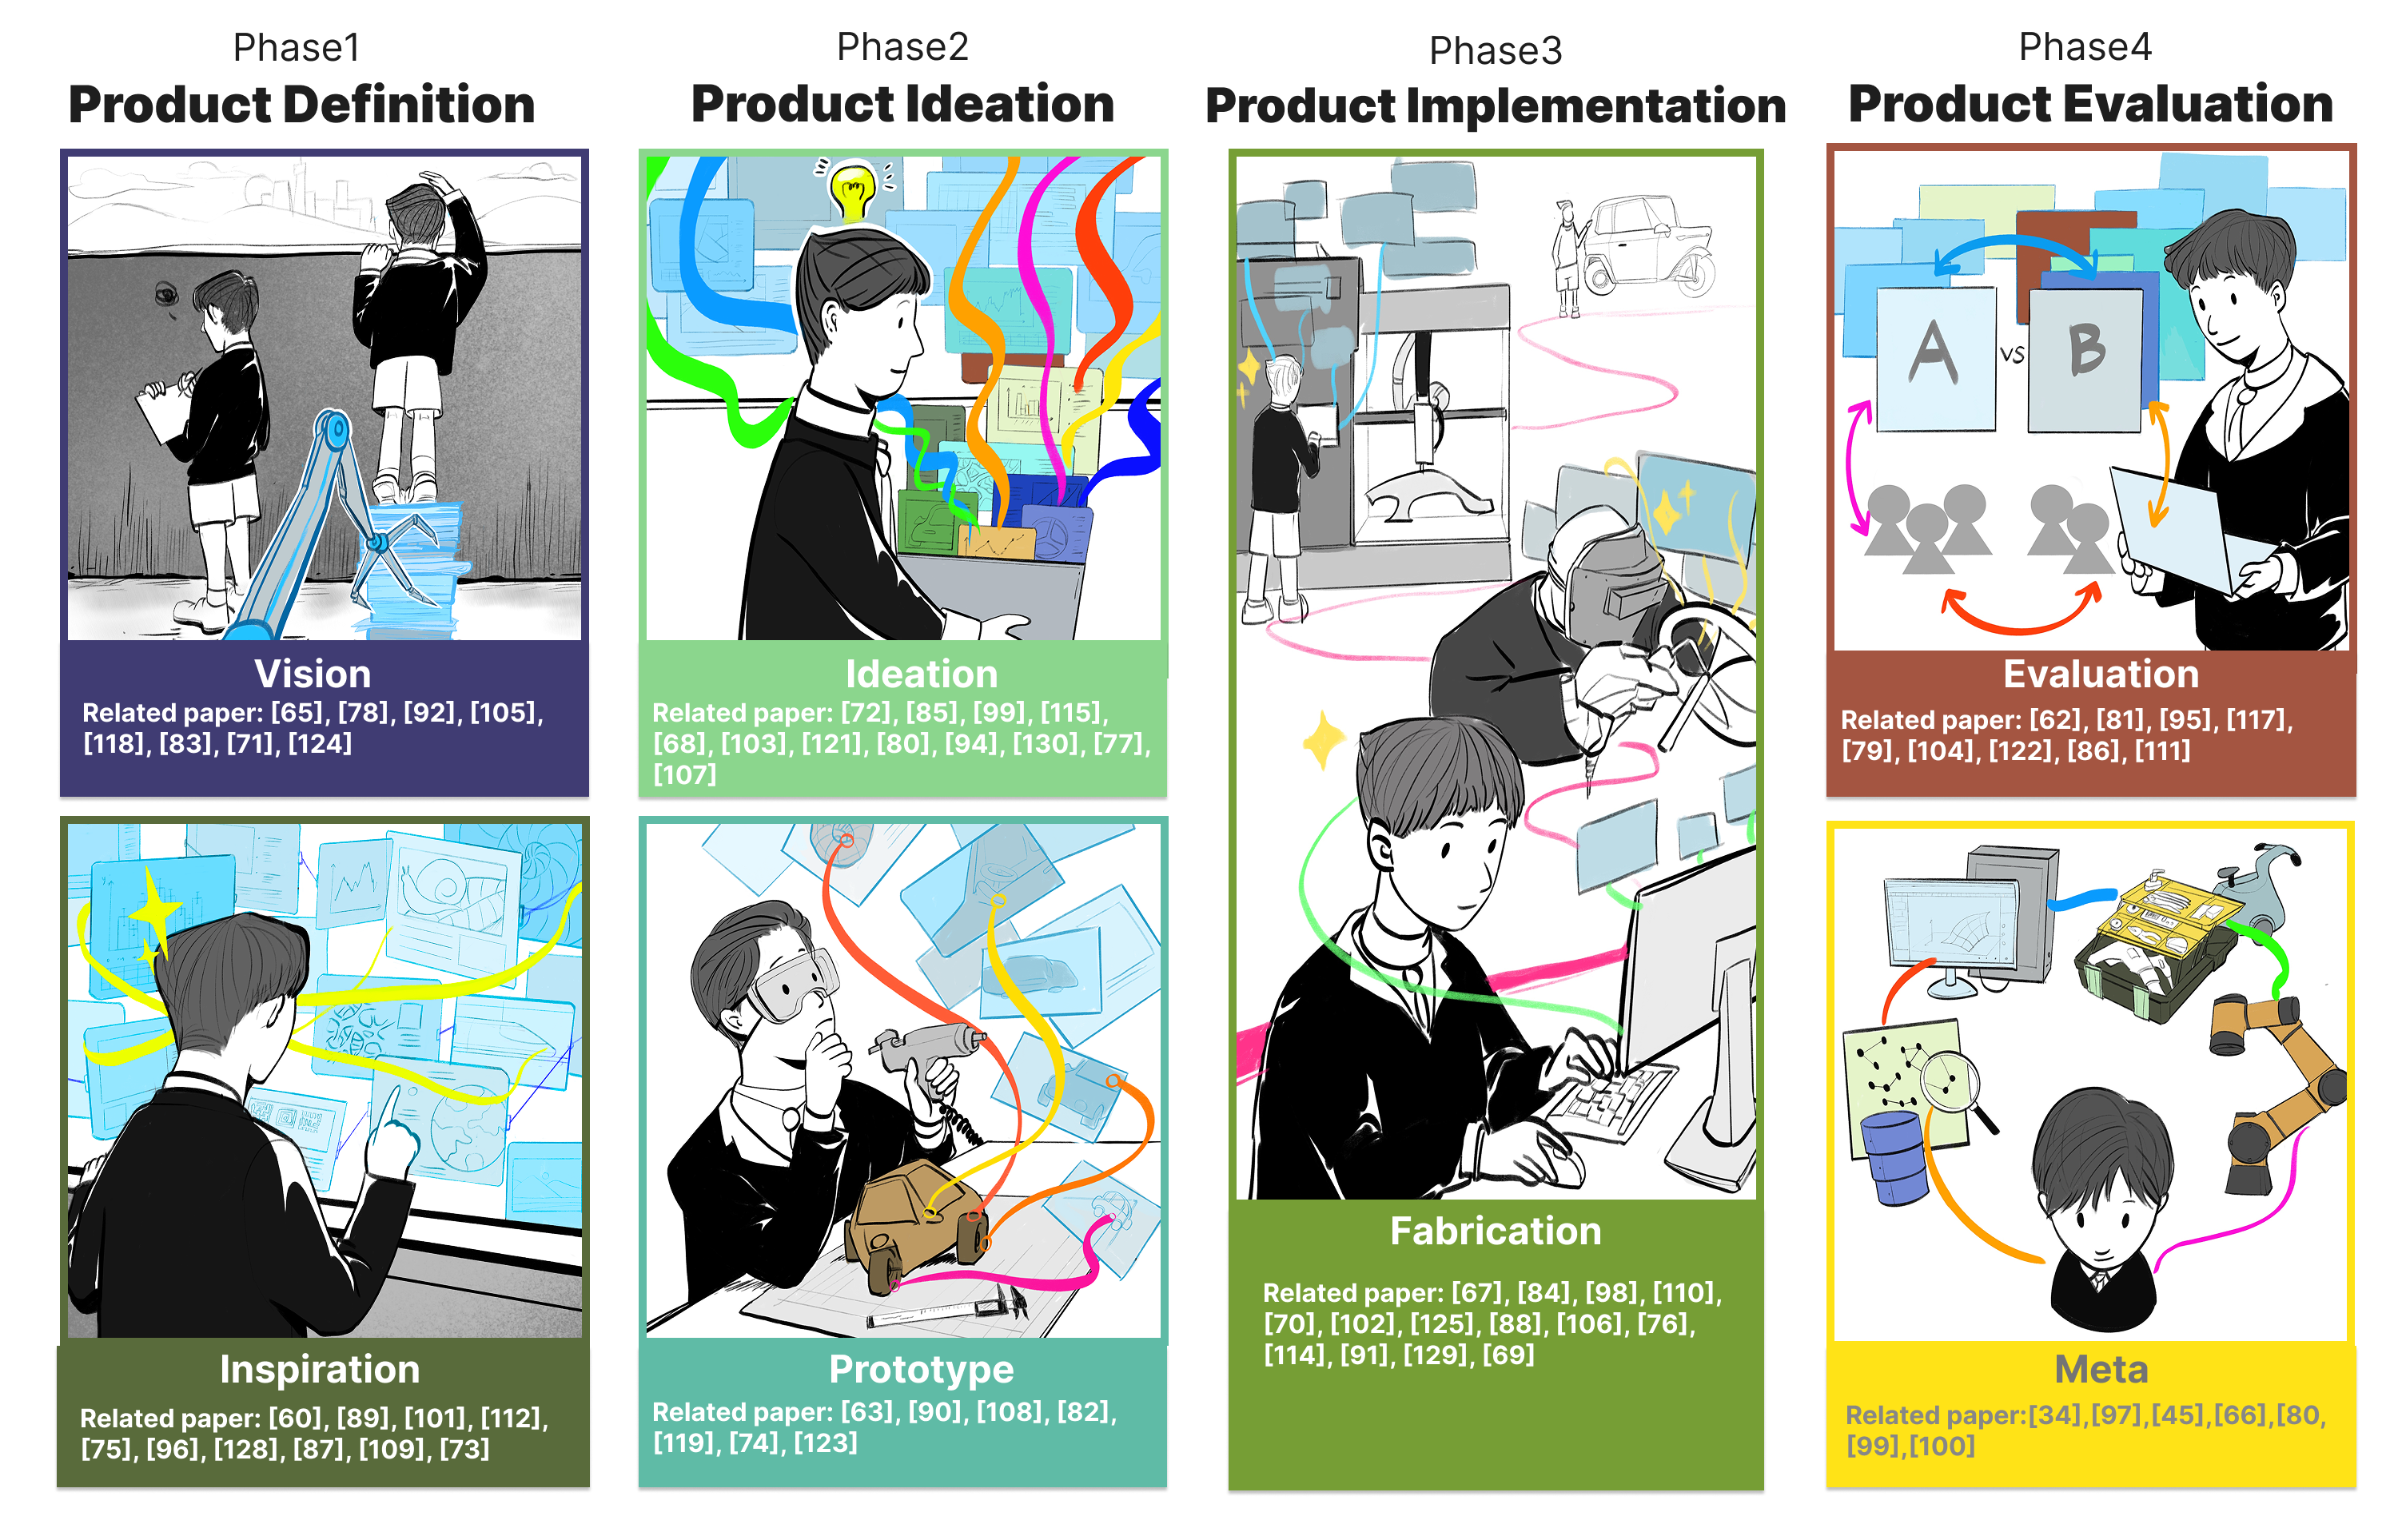
\includegraphics[width=1\linewidth]{Figures/CreateProcess.png}
    \caption{To elaborate on the technical mediation value\cite{smits2019values} of Design-by-Analogy (DbA) across different segments, we employ comic illustrations to visualize its abstract functions throughout various design phases. Based on the maturity of ideas, the entire process is categorized into 4 primary stages and 7 iterative sub-processes: in \textbf{\textit{Vision}}, the illustration adopts a metaphor where individuals standing behind a wall are unable to perceive distant landscapes, symbolizing that DbA can act as a knowledge-based foundation to elevate human cognitive horizons. In \textbf{\textit{Inspiration}}, it portrays that those positioned at a sufficient height can access diverse sources of inspirational stimuli. In \textbf{\textit{Ideation}}, DbA facilitates the screening of multiple inspirational stimuli and guides operators to independently converge heterogeneous stimuli into a coherent idea. In \textit{\textbf{Prototype}}, DbA recommends professional practices to support the optimization of ideas. In \textit{\textbf{Fabrication}}, DbA technology can be integrated into relevant software and hardware systems to provide experiential assistance and knowledge transfer for specific operational processes. And both \textbf{Evaluation} and \textbf{\textit{Meta}} stage are designed to assist operators in achieving experiential migration.}
    \label{fig:Create Process}
\end{figure}





%我们用漫画插图的形式表达每个部分DbA技术可以起到的技术中介价值,展现了在各个设计阶段,Design-by-Analogy技术可以起到的抽象作用。按照idea的成熟度,我们划分了四个主要阶段和迭代的7个子过程。其中vision阶段,插图使用站在墙后无法看到远处风景的隐喻,暗示dba可以作为垫起人类认知视野的知识地基,inspiration阶段,站的足够高的人可以接触多样化的灵感刺激,ideation阶段则是dba辅助人类对多种灵感刺激进行筛选,引导操作者自主将多类型的刺激收敛为一个idea,prototype阶段,dba则推荐更多专业做法辅助优化idea,fabrication阶段,dba技术可以嵌入在相关软件和硬件中对具体实操进行经验辅助和迁移,evaluation阶段和meta阶段也将辅助操作者进行经验迁移。




















%---------------------draft---------



%1.这一阶段,创意任务的主要内涵是定义问题,发现真正的结构性问题所在,而非有一个statement就直接开始设计,新的设计挑战往往面临:(1)武断的设计出发点会导致设计结果偏离初始目标,也会导致经济和投资的亏空和损失,本阶段可以设计师在设计前期节省成本、深刻溯源及因果推断。(2)所需产品或设计已经有其他人进行开发和解决了,找到真正的痛点问题才能真的解决问题,比如在这一设计研究中xxx得到证实,大约有xx的社区纠纷的主要矛盾并非人与人,而是环境设计的问题,这样的归因链路仰赖丰富的环境设计经验和人类学经验,是很难被没有设计背景的任意学科工程师所找到的,这就需要相关的领域知识经验库。(3)在启发阶段,类比设计可以提供更开阔的思路,更加全面的语料库检索,打开用户的思路,xxx证明会有启发帮助能力,这个阶段的内容会是多样的,零散的,分布在多个远距离领域尚未聚焦的状态,是混沌的但是充满可能性的,未经用户的内在知识运作的。

%2.研究表明,80%的设计成本在构思阶段即被锁定。大量商品耗材、能源浪费及不可持续性设计产物(如无效设计与废弃方案),可借由经验体系与智能类比设计系统辅助在本阶段规避。DbA通过「问题定义-启发收敛」框架支持用户生成完整方案,该方案具有收敛性、目标聚焦性,且深度融合用户内在经验与核心需求。至原型阶段,用户可对特定方案进行深度迭代优化(如结构修正、流程改进、美学升级),系统将启动领域适配型类比推荐机制,提供近距离参考案例的细节处理技巧、失效预防策略及领域知识迁移路径,支撑方案的精细化打磨。



%3.这一阶段,创意任务的主要内涵是围绕着某一具体想法进行实际的操作、落地产出和标准化生产。市面上观点认为类比或基于认知的方法仅仅只能在创造阶段的前期进行辅助,这一观点暗含一种假设,即,致力于研究物理制造的研究者们默认在实际操作阶段的经验难以或不能被转化成结构化的知识,因为具体操作阶段往往是case by case的,其个性和特异性较大。这一认识潜在造成了许多经验化的操作流程的数据的根本性模糊,如,本可以被大范围复现的实操工艺,小众制造技艺及实践文化,被从制造者的经验上和认知上不加以定量记录,模糊记录或者不认为可以定量记录的手工实操中遭遇忽略甚至遗失。所以基于类比设计的制造阶段的经验转移可以说是一个尚未被大面积开发的研究领域,时常被急于落地的制造者们主动忽略。我们认为在此阶段类比设计方法有着大量潜力。因为自动化的,标准化的执行和生产在流水线中基本完全仰赖大型智能制造机械,只要耗材经过可被计算的软件和机器进行生产,那么就可以被经由可推理,可结构化映射的类比设计方法增强设计决策和创造力。同时,小众的手艺和文化的传承也仰赖标准化,精确的制造参数和工艺流程来进行记录和传承,这些经验是文化档案,也是可被迁移和转化用于新的设计的类比设计所需数据。




% \textbf{\underline{Production.}}
% %这一阶段与上一阶段不具有清晰的界限,更偏向于投入流水线之后的具体操作,本阶段使用类比设计技术的全流程整合可以辅助用户实现自动化的操作。


\section{Applications}
%按应用领域分了,再统计一下
This section introduces prevalent application domains where Design-by-Analogy can deploy and examines domain-specific challenges, focusing on three sectors: Creative Industries, Intelligent Manufacturing, Education and Service Industries. Although DbA methods could theoretically support creative processes in other domains (e.g. pharmaceutical design, algorithmic design), this study exclusively addresses end-to-end applications that directly serve users and solve practical problems.
% 在本节中,我们介绍了常见的类比设计应用领域,并讨论了每个应用领域特有的分析挑战。这包括三个领域:创意工业, 智能制造,以及教育及服务工业。虽然其他应用领域也可使用design by analogy方法进行创造过程的辅助(如医药领域的药品设计,生物化学领域中的基于类比启发新化合物形式,算法设计领域的根据类比设计新算法),但它们不在本文的讨论范围内。在本节中,我们关注可以直接服务用户,解决实际的问题的端到端产业和行业上的应用。
\subsection{Creative Industries} %【13篇】
In 1998, the UK Department for Culture, Media and Sport (DCMS) defined ``creative industries'' as \textit{``Based upon activities which have their origin in individual creativity, skill and talent, and as having the potential for wealth creation through the generation and exploitation of intellectual property}\cite{miles2008hidden}. '' The Design-by-Analogy Application cases collected in this paper include creative writing, graphic design, product design, 3D modeling, animation, web design, scientific tasks, data visualization and the function of computer aided design system which related to computer graphics development, researchers using DbA methods toward different domain challenges, excluding film and music. Industrial outputs rely primarily on computational technologies and structured data, barring noncreative factors(e.g., political or force majeure events) \cite{miles2008hidden}. Our investigation identifies two core challenges for novices the create process: (1) The prevalent high technical and aesthetic barriers in software requiring experience-creativity synergy, frequently preventing concept realization\cite{hsueh2024counts}. It is common for novice designers to have an idea but be unable to implement it through software or implement it imperfectly. (2) Trendy aesthetic, emerging cultures, and edge-cutting concepts is uneven dissemination, due to the universal aesthetic knowledge bases, creative knowledge bases, design theory bases, and etc. still lacking of universal tool embedded. The effective integration of DbA technologies can: (1) Enable beginners and professionals to rapidly access cutting-edge design knowledge (patent details, case imagery, semantic inspiration). (2) Facilitate precise transfer of knowledge, styles, and content to enhance creative representation and efficiency. (3) Stimulate creator innovation through intrinsically guided knowledge exploration, thereby reinforcing creative autonomy. Academic research\cite{srinivasan2024improving, masson2025textoshop, warner2023interactive, chen2024beyond,wang2024reelframer, zheng2024disciplink,yan2023xcreation,chen2021umitation, kittur2019scaling, goucher2019crowdsourcing, han2018computational, lin2025inkspire, song2020exploration} has proposed domain specific solutions detailed subsequently.


%1998年,文化、媒体和体育部(DCMS)将创意产业定义为基于源自个人创造力、技能和天赋的活动,并且具有通过创造和开发知识产权来创造财富的潜力。本文所收集到的类比设计案例,涵盖创意内容写作、平面设计、产品设计、3d模型设计、动画设计、网站设计、科研任务、数据可视化设计及相关计算机辅助设计软件(CAD)的相关图形学功能开发等,尚未涵盖电影、音乐。本行业的工业化产出几乎仰赖于计算机技术和结构化的数据,除了非创造过程以外的其他因素如政治、不可抗力因素等,我们调查了相关研究发现本行业初学者在创造过程中的一些痛点,其中:大量的软件有着高使用门槛和美学门槛,这些门槛往往需要经验和创意的共同加持,新手设计师有一个idea但无法通过软件进行实现或者实现的不完善的情况是常态。第二点,潮流美学趋势、新兴文化、前沿理念在知识密集的区域会大面积传播,普适的软件内嵌美学知识库,创意知识库,设计数据库等通过类比设计这一机制可以促进地区的文化平权。类比设计的技术的有效整合可以(1)使不同知识深度的操作者可以快速链接到前沿知识,如相关的专利的具体设计细节,案例图片,近距离或远距离的词语启发等;(2)基于结构化映射计算,软件自动化的对知识、图形,风格等内容进行映射和迁移,从而辅助操作者更准确和更高水平的展现创意,提升完成度和效率,人辅助;(3)创意类比可以激发作者的创造力,根据作者的内在经验和知识来驱动外部知识的发散方向,这有利于保护和增强作者的内在价值和主体感。在学术研究中,学者们已经使用了各种解决方案来应对这些挑战【13篇】【1、4、9、10、11、13、15、32、42、43、45、50、71、】,我们根据应用领域的不同在下文对其方法进行详细描述。


%In creative product design, high cognitive load and design fixation\cite{moreno2015step} challenge ideation. \textbf{\textit{Crowdsourcing Inspiration}} employs crowdsourcing and text mining to extract semantic patterns from solution databases, visualizing word frequency distributions\cite{goucher2019crowdsourcing, kittur2019scaling}. \textit{\textbf{Analogilead}} enables chunk-based recombination for scalable analogical exploration\cite{srinivasan2024improving}. \textit{\textbf{The retriever}} proposes 16 ontology-based relations. By abstract the ontology relations, it retrieving and constructing an ontology or its substructure\cite{han2018computational}.
%在产品创意设计领域,一个idea的诞生需要保证创造性的同时考虑大量复杂性因素,这一过程的认知负荷很高,且极容易陷入设计固定,【42】通过众包方法得到关于12个设计问题的大规模解决方案文本,并且对解决方案进行文本挖掘,以沿频率域提取单词,映射为语义距离,并可视化展示给设计师增强创造力,【43】Kittur等人利用人群协作和AI来扩展类比创新,通过将类比过程分解为抽象、搜索和应用三个步骤,并分配给不同的人类和机器处理器,从而在这一阶段解决设计固定。【1】analogilead则通过设计师自主的组块和重组扩展类比规模,回应这一挑战。【45】The retriever 提出了16种基于本体的关系,通过在不太熟悉的本体(目标本体)中基于已知术语 C 以及从熟悉的本体(基础本体)中的 A:B 抽象出的本体关系,检索未知的 X 或多个 X,来构建一个本体或本体的一部分,激发创意。
%For graphic and 3D design, style modification typically requires rebuilding geometries from foundational elements. \textit{\textbf{VST}} allowing designers to define element correspondences and style attributes\cite{warner2023interactive}.
%automating vector graphic style transfer while preserving artistic intent of designer
%在平面设计和3d设计领域,图形和模型风格的改变往往意味着操作者需要弃用之前做的内容并重新在软件中从点、线、面开始制作新的形状,【9】warner等人在尊重设计师品味以及风格迁移所固有的主观性的同时利用自动化方法,设计师在其界面上可以调整跨设计元素的对应关系,并自定义要更改的风格属性,通过生成式人工智能迁移和映射矢量图形的风格,优化冗余步骤。
%In creative software development, transferring experience based on culture, user behavior, interaction, etc. often leads to product innovation. \textbf{\textit{Textoshop}} innovates by transferring image editing logic to text manipulation: words as pixels, sentences as regions, and tone as color\cite{masson2025textoshop}.
%This application enabling novel textual operations through transfered interaction
%在计算机辅助创意的软件开发过程中,基于文化、用户行为、交互等内容进行经验的迁移往往会带来产品的创新,【4】Textoshop利用图片编辑的逻辑迭代文字编辑,他们将单词视为像素,句子视为区域,语气视为颜色。对文本的直接操作可移动、缩短、扩展和重新排列文本;工具可改变数量、时态和语法;在色调选择器中,颜色映射到沿三个维度探索的语气;而图层则有助于组织文本并进行版本管理等。
%In journalistic content creation, the rapid expansion and transformation of content forms usually require the switching of diverse disciplinary skills. \textit{\textbf{ReelFramer}}, converting print articles into short video scripts using 3 different narrative frameworks\cite{wang2024reelframer}. \textbf{\textit{Xcreation}} \cite{yan2023xcreation} transform text-to-illustration workflows through editable entity relationship graphs.
%在新闻内容创作领域,新闻内容形式的快速扩展和转化通常需要差异性的学科技能切换,wang等人【11】提出三种适用于短片的叙事框架,这些框架既适应社交媒体规范,又保留了新闻价值,每种框架在信息和娱乐之间有着不同的平衡,他们的ReelFramer可帮助记者将印刷文章根据规则映射为脚本和故事板。相似的模态转换,还有在插画设计领域中的文字模态到图片插图模态的转换,yan等人【15】整合了一个可解释的实体关系图,以直观地表示图片元素及其之间的关系,从而将文字到图片的这种映射规则可视化成为具有边、节点的图,用户可以编辑,提高映射的可用性。
%For web design, front-end UI development involves highly repetitive DOM modifications requiring constant contextual adaptation. \textbf{\textit{Umitation}} optimizes repetitive DOM adjustments by recording UI behaviors on source sites and mapping changes to target elements, contextualizing design adaptations.
%在网页设计中,大量的前端ui文档对象模型的变化设计工作是重复性高且需不断根据情境调整的,一次ui行为更改和调整意味着复杂的底层内容变动,基于经验、可行性和情境进行设计则会提升效率,umitation【32】帮助设计师提取、编辑并将前端 UI 行为示例适配到目标网站的系统。通过首先在源网站上指定一个或多个源元素,然后通过与它们交互来记录其行为。umitation将自动捕获文档对象模型(DOM)的变化并将其映射到目标网站上的合适元素,帮助明确设计师所需的ui行为。
%In data visualization, achieving user comprehension of complex data and developing more comprehensible representations is the primary objective. \textbf{\textit{AnalogyMate}} employs proportional text and graphics for data analogy to convey complex numerical values, units, and concepts in ways that enhance comprehension\cite{chen2024beyond}.
%在数据可视化设计中,用户对复杂数据的清晰理解是首要目标,而给复杂数据寻找更具理解力的表征是难点,chen等人【10】利用与数据比例一致的文字和图像来进行数据类比,他们定义了数据类比设计的多种维度,致力于将复杂的难以理解的数值、单位、概念以更能增加理解的方式传达给读者。
%In interdisciplinary research, cross-disciplinary information retrieval involves terminology discrepancies and integration of vast content. \textbf{\textit{DiscipLink}} assist users in query formulation, automatically expanding queries using domain-specific terms, extracting topics, and establishing research connections\cite{zheng2024disciplink}.
%在跨学科科研中,跨学科的信息搜索意味着术语差异,大量内容的整合对比,陌生学科的高度分散的知识中进行梳理是一项重大挑战,DiscipLink【13】从辅助用户提问出发,根据特定学科术语自动扩展查询、从检索到的论文中提取主题以及与问题之间的联系,帮助用户进行跨领域的术语转换和科研内容映射。




\subsection{Intelligent Manufacturing} %智能制造,会写生物设计,机械设计,农业,电子电路还有机器人什么的(制造的)【15篇】
In the Industry 4.0, intelligent manufacturing is defined as an advanced mode that utilizes artificial intelligence, the Internet of Things, cyber-physical systems, and related technologies to transform traditional manufacturing resources into intelligent objects with perception, decision-making, and collaboration capabilities. This enables data-driven flexible production for mass customization.\cite{zhong2017intelligent, jiang2022data, li2017applications}. We documents DbA applications including: knowledge-based design inspiration\cite{kang2025biospark}, case-integrated design-to-manufacturing lifecycle system\cite{thomas2013extending, schulz2014design}, case-based cyber-physical system\cite{gonzalez2018energy}, and process-oriented intelligent knowledge transfer\cite{emerson2024anther}. These span manufacturing method design\cite{luo2019computer}, product innovation\cite{liu2023smfm}, smart sensor/wearable device development\cite{hong2024fishbone}, plastics processing\cite{khosravani2022intelligent}, chemical/pharmaceutical synthesis\cite{coley2019robotic}, and agriculture\cite{zhai2020applying}. DbA further empowers industrial upgrading through manufacturing case libraries and design databases by: (1) Transferring cross-domain knowledge to product manufacturing methods, supporting innovative resource utilization; (2) promote lifecycle servitization of physical manufacturing resources through AI-assisted manufacturing decisions; (3) provide replicable conversion pathways for niche manufacturing techniques, fostering innovation within Community Of Practice(COP) and fostering archival and transform of ambiguous data\cite{zhong2017intelligent, kusiak2000computational, jiang2022data}. Deep exploration and integration of this mechanism in intelligent manufacturing offers beginners heuristic resources and assists experts in enhancing complex problem-solving through cross-scenario functional and structural migration. It optimizes implementation of modular production units, flexible logistics planning, and mass personalized customization\cite{li2017applications}, while improving energy and resource allocation to advance sustainable development. Research in this domain includes\cite{kang2025biospark, emerson2024anther, zhai2020applying, fan2014fractal, luo2021guiding, schulz2014design, liu2023smfm, luo2019computer, hong2024fishbone, khosravani2022intelligent, you2018design, thomas2013extending, coley2019robotic, gonzalez2018energy}.
%在工业4.0背景下,智能制造可定义为依托人工智能、物联网、信息物理系统等技术,将传统制造资源转化为具备感知、决策与协作能力的智能对象,通过数据驱动与柔性化生产实现大规模定制的先进制造模式。本文收集的类比设计相关应用涵盖基于知识库的设计灵感启发、基于案例集成设计到制造全生命周期、基于案例的信息物理系统、基于知识的流程规划、基于工艺的智能知识迁移等,包含的应用领域包括制造方法设计,产品创新设计,智能传感器与可穿戴设备的设计与制造,塑料加工,化学合成与制药、农业等行业。类比设计在该领域的应用可进一步赋能产业升级,通过构建制造案例库与设计数据库:(1)能将生物结构、工程专利等跨领域知识迁移至产品制造方法中,促进制造资源的创新应用;(2)基于工艺规划经验与知识数据库,结合AI辅助制造决策,推动实体制造资源的全生命周期服务化;(3)为小众制造技艺提供可复刻的转换路径,促进实践制造社区的创新和模糊数据存档。在智能制造领域深入探讨这种机制并集成,可为初学者提供工艺参数、经验库等启发资源,帮助专家通过功能、结构等内容的跨场景迁移提升复杂问题的解决效率,依托创意类比设计优化模块化生产单元设计、柔性物流路径规划,大规模个性化定制等创新场景的落地,优化能源和资源分配,促进智能制造行业的可持续发展。在学术研究中,学者们已经使用了各种解决方案来应对这些挑战【2,3,12,30,41,52,57,61,62,64,67,72,77,80,82】,我们根据应用场景的不同在下文对其方法进行详细描述。
%---------------------------
%智能制造行业关注的三个内容(1)流程、加工、工艺数据实时采集的完整性(如温度、振动、能耗等);(2)实体可制造资源的全生命周期服务化。(3)柔性化、个性化、定制化生产的需求在大幅增加。



%在农业智能化领域,

% 根据文档内容及所提供的文章标题,可对各研究所属行业及解决的智能制造问题分析如下:  

% 1. **《将基于案例的推理和基于学习的适应策略应用于葡萄种植中的灌溉调度》**:  
%    所属行业为农业智能化领域。其通过案例推理与学习策略优化灌溉调度,对应文档中智能制造“数据驱动决策”与“自适应控制”的技术特征,解决了农业生产中水资源高效利用的实时决策问题,类似于制造系统中基于历史数据的工艺参数优化(如文档中提到的RFID实时数据驱动生产调度,)。  

% 2. **《通过实例进行设计与制造》**:  
%    属于制造业设计领域。该研究利用实例推理辅助设计与制造,契合文档中“智能设计”与“案例库应用”的方向(如提到的基于CAD/CAM的智能原型系统),解决了产品设计中知识迁移效率低的问题,实现设计经验的复用与创新。  

% 3. **《基于功能案例建模和生物TRIZ的生物启发式设计中的设计类比》《基于SMFM的创新产品概念设计类比检索工具》**:  
%    归属产品创新设计领域。两者通过生物类比与功能建模推动设计创新,对应文档中“类比设计辅助制造”的思路(如提到的多智能体协作与跨领域知识映射),解决了传统设计中创意生成与功能优化的瓶颈,类似于将生物结构类比至机械部件设计的跨领域应用。  

% 4. **《受鱼骨和荨麻纤维启发的高灵敏度、宽传感范围可拉伸应变传感器及其在可穿戴电子设备中的应用》**:  
%    属于智能传感器与可穿戴设备制造领域。其通过生物启发的材料设计提升传感器性能,对应文档中“智能对象感知能力”的技术要求(如提到的RFID与传感器集成实现生产资源感知),解决了智能制造中实时数据采集的精度与范围问题,为柔性制造提供硬件支撑。  

% 5. **《基于智能知识的系统以改进注塑成型工艺》**:  
%    属于塑料加工制造领域。该系统通过智能知识管理优化注塑工艺,对应文档中“AI驱动的工艺优化”(如提到的AI在生产流程监控中的应用),解决了注塑成型中参数优化与质量控制的复杂性问题,实现工艺的自适应调整。  

% 6. **《类比设计:一种用于岩土工程的特征树方法》**:  
%    属于土木工程智能化领域。其将类比设计应用于岩土工程,类似于文档中“跨领域知识迁移”的思路(如提到的制造系统多智能体协作),解决了岩土工程中复杂场景的设计决策问题,为智能制造中的模块化设计提供方法论参考。  

% 7. **《扩展和自动化用于需求生成与分析的系统理论危害分析》**:  
%    属于制造系统安全与需求分析领域。其通过自动化危害分析提升系统可靠性,对应文档中“智能制造系统安全性”的考量(如提到的云计算安全挑战),解决了生产流程中潜在风险的预判与需求分析效率问题。  

% 8. **《一个由人工智能规划驱动的用于有机化合物流动合成的机器人平台》**:  
%    属于化学合成与制药制造领域。该平台通过AI驱动机器人实现自动化合成,对应文档中“智能装备与自主控制”的技术方向(如提到的智能机器人在IMS中的应用),解决了有机合成中流程复杂、自动化程度低的问题,推动制药制造向智能化转型。  

% 9. **《基于案例推理策略的能源优化》**:  
%    属于工业能源管理领域。其通过案例推理优化能源分配,对应文档中“制造资源高效利用”的目标(如提到的ICT助力制造业节能),解决了工业生产中能源消耗的优化调度问题,实现智能制造中的绿色生产需求。  

% 这些研究从不同维度呼应了文档中智能制造在“数据驱动决策、跨领域类比设计、智能装备优化、资源服务化”等方面的技术需求,通过案例推理、生物启发、AI规划等方法,分别解决了各行业中知识迁移、工艺优化、实时感知、能源效率等具体问题,为工业4.0背景下的智能制造提供了多元化的解决方案。

\subsection{Education and Service Industries}%会写一些类似服务业的内容,金融类比,服务流程类比也有一些文章【14篇】
Analogical reasoning, recognized as fundamental to learning\cite{winston1980learning} with deep philosophical roots and extensive mathematical applications, enjoys broad pedagogical exploration supported by substantial theoretical and empirical research\cite{bettin2023pedagogical}. We documents DbA applications in education, distinct from pure analogical reasoning, which structurally scaffold analogical application in educational contexts\cite{winston1980learning, bettin2023pedagogical}. By systematically retrieving knowledge, experience, and data, then transferring them via domain-specific mapping rules to target scenarios, these tools empower educators to rapidly leverage adapted resources for advancing students' conceptual understanding, metacognition, and interdisciplinary exchange\cite{karunathilaka2025intuit, chen2024BIDTrain, ball2019advancing}.
Within service industries, DbA facilitates transactional innovation across cultures, domains, services, and communities by enabling communication, collaboration, and co-creation. Such tools map and migrate tacit knowledge through domain-specific rules, allowing practitioners to integrate existing expertise with novel insights while addressing critical challenges\cite{moreno2014analogies, lee2020customized}: (1) Leveraging shared methodologies (e.g., touchpoint analysis, stakeholder mapping, service blueprints\cite{stickdorn2012service}) despite service design's case-specific nature, enabling cross-scenario inspiration through experience repositories; (2) Embedding resolved complexities from other contexts into service design applications to enhance practical efficacy; and (3) This field demands rigorous design evaluation, and DbA based assessment holds significant potential for evaluating and predicting service efficacy. Research in this domain includes\cite{chen2024BIDTrain, kim2023star, dougan2022predicting, jiayang2023storyanalogy, cao2025medai, shao2025unlock, bettin2023pedagogical, Ju2025toward, karunathilaka2025intuit, vattam2011dane, la2020designing, moreno2014analogies, lee2020customized, lupiani2017monitoring}.
%类比推理被认为是学习的本质,其深厚的哲学研究根基、在数学科学中的应用,使其在教育学界的探索十分广泛,有着大量的理论与实践研究。本文检索到的类比设计工具,区别于单纯的类比推理,旨在结构化的辅助教学场景中的类比应用,通过系统检索到的知识、经验、数据等,经由特异性映射规则迁移到具体的教育应用场景中,使教育工作者可以快速使用迁移好的知识推动学生的概念学习、元认知、理解能力等,并促进学科间交流。
%在服务工业领域,类比设计被应用于促进跨文化、跨领域、跨服务、跨社区的事务性工作创新,通过支持交流、协作与共创机制驱动价值创造。该类工具将模糊知识、经验等抽象内容基于领域特定规则进行映射迁移,赋能事务性工作者快速融合经验与新知开展工作,并针对性解决以下核心问题:1)尽管服务设计具有强情境依赖性(case by case)与在地特异性,但共性要素依然存在(如触点分析、利益相关方分析、服务蓝图等流程化方法),该层面可依托经验库实现推荐机制、灵感激发与跨场景映射;2)特定复杂性问题可能已在其他情境中被高效解决,通过将既有经验与细节嵌入服务设计理论框架及流程化交互支持系统,可强化类比设计的实践效能;4)本领域对设计评估需求很高,基于类比设计评估和预测服务效能具有很大潜力。


%
\begin{figure}
    \centering
    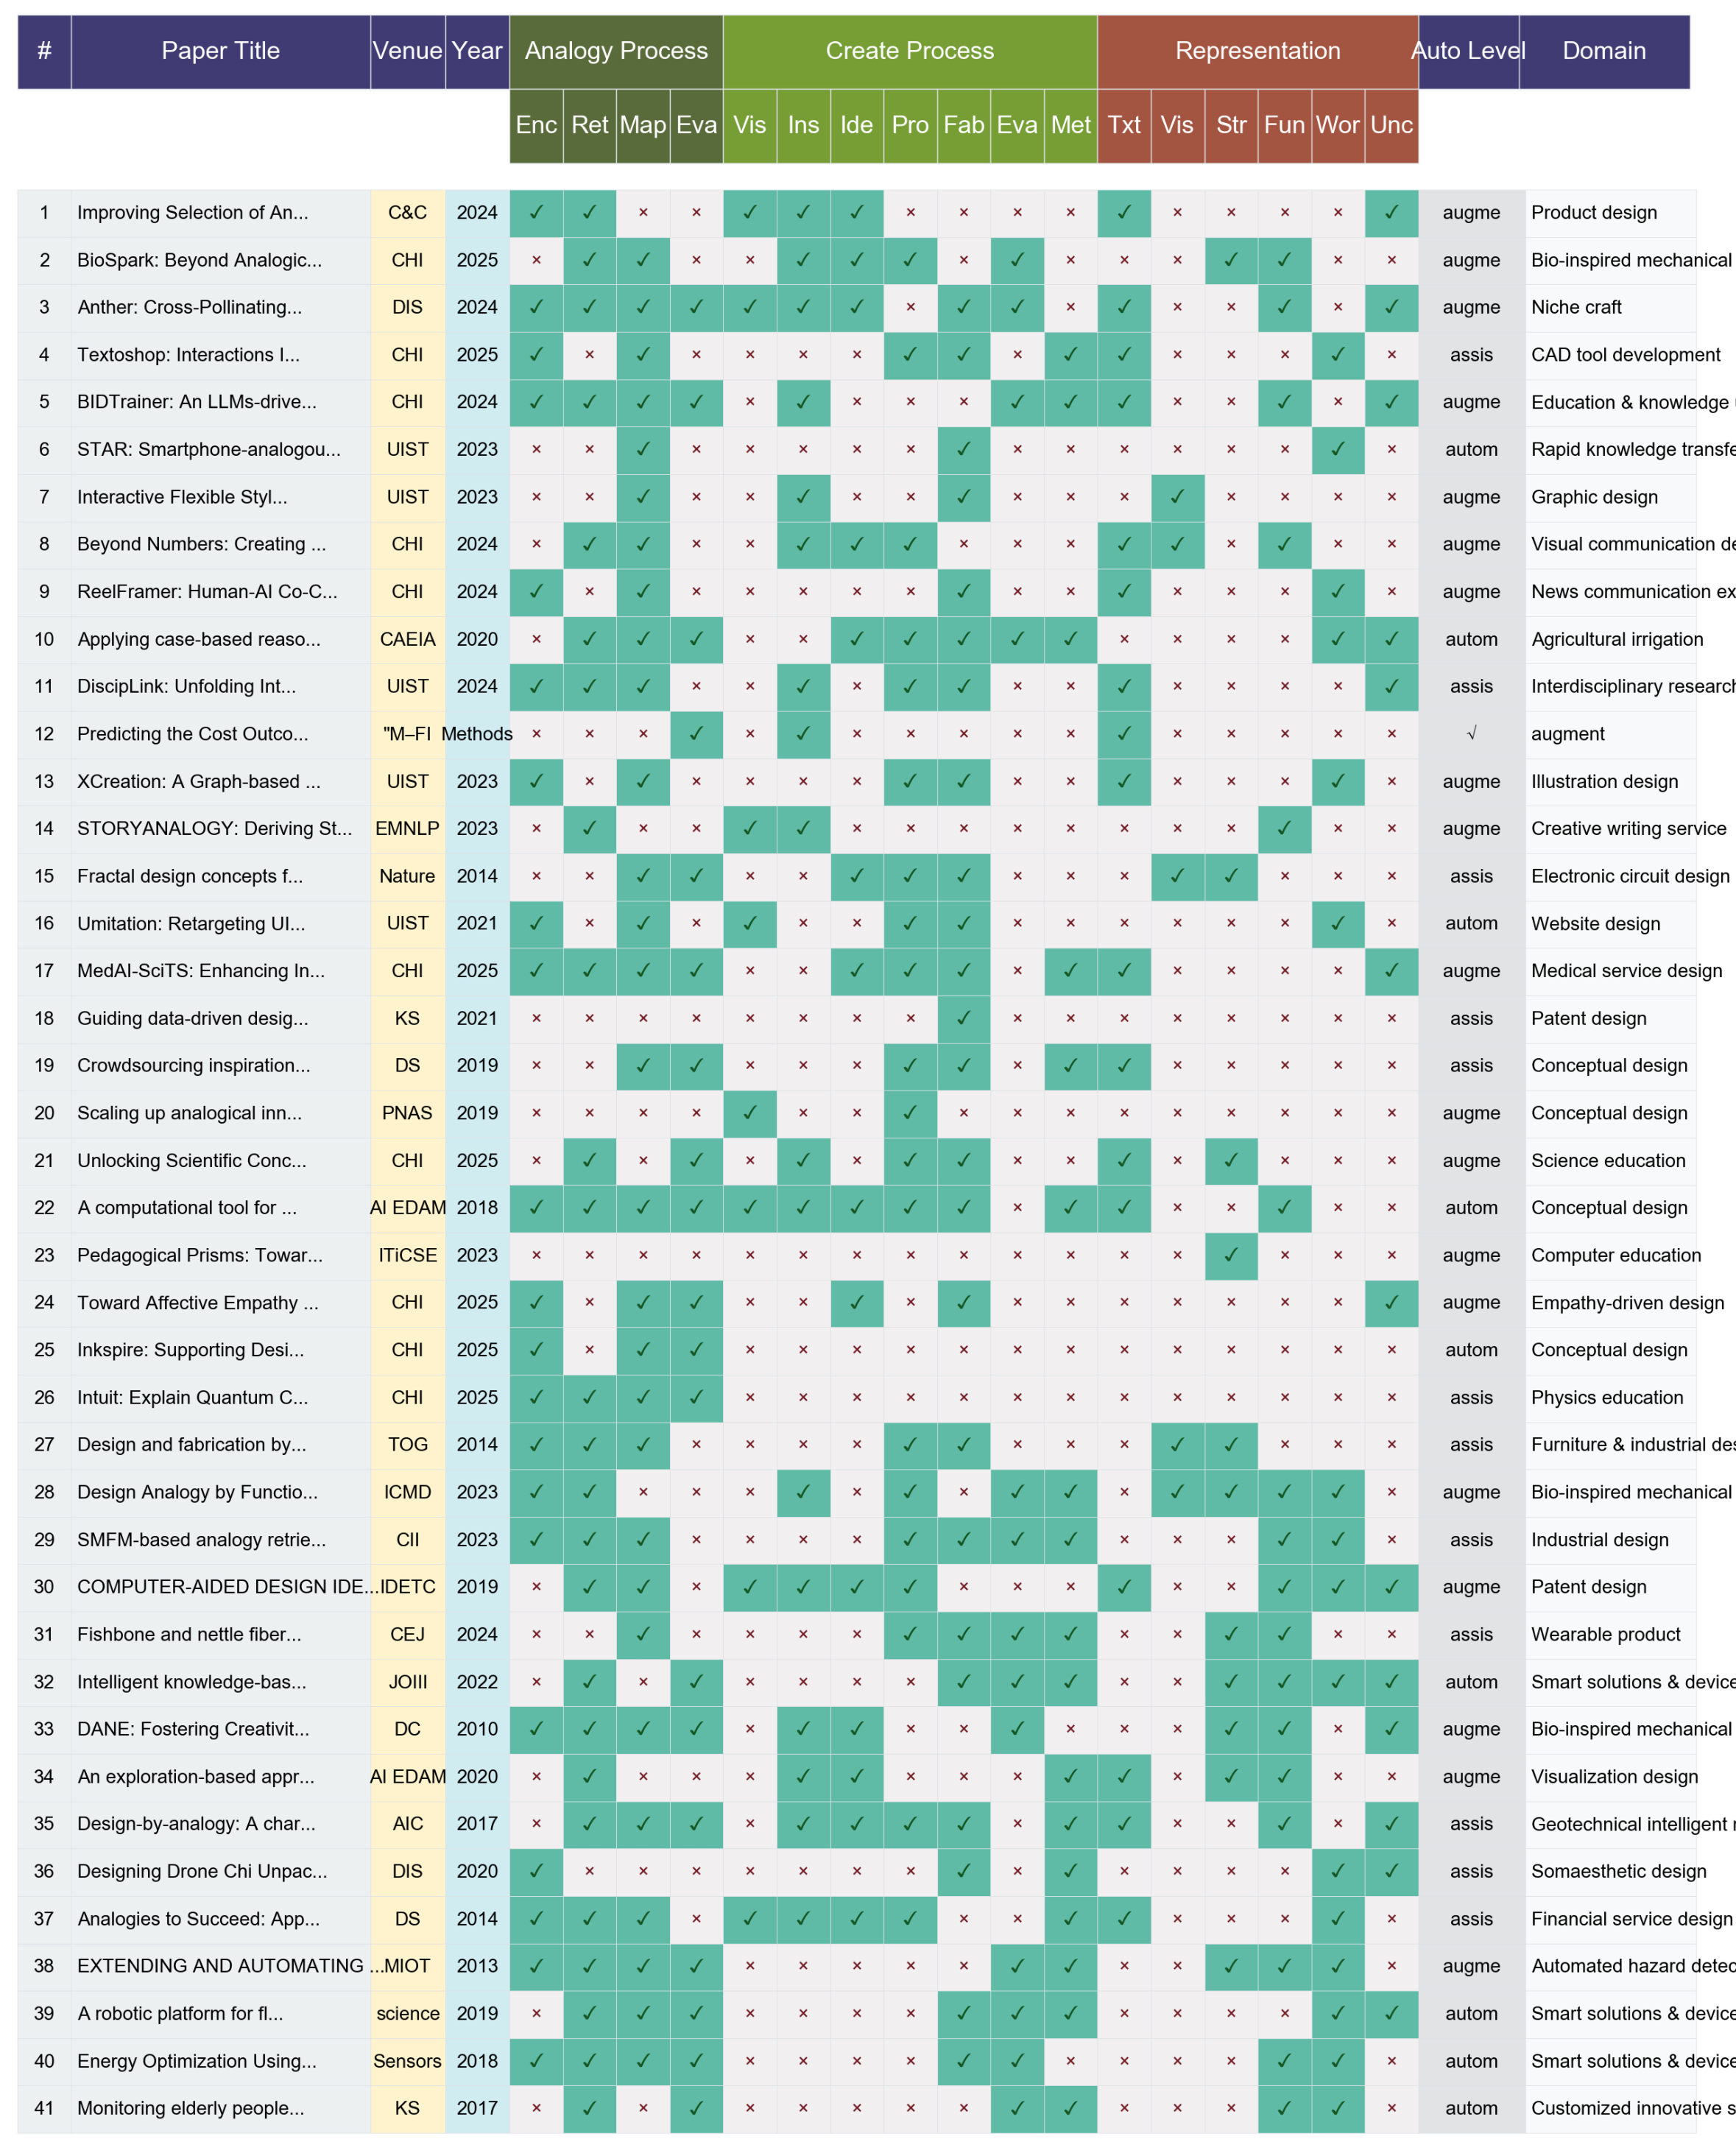
\includegraphics[width=1\linewidth]{Figures/complete_41_papers_presentation 2.png}
    \caption{This figure visualizes a taxonomic matrix consisting of 42 representative publications in the field of AI - enabled analogical design from 2010 to 2025. The x - axis represents different application domains (for example, communication design and fabrication), while the y - axis distinguishes between two technological orientations: Augment and Automate. The publication year encodes the temporal distribution, and visual markers indicate the intersections between domains and technologies. This matrix provides a comprehensive overview of the research trajectories and methodological focuses in the field.}
    \label{fig:enter-label}
\end{figure}














%-------------draft--------------------------

%在工业4.0背景下,智能制造可定义为依托人工智能、物联网、信息物理系统等技术,将传统制造资源转化为具备感知、决策与协作能力的智能对象,通过数据驱动与柔性化生产实现大规模定制的先进制造模式。本文收集的类比设计相关应用涵盖基于知识库的设计灵感启发、AI优化适应性制造决策、基于案例集成设计到制造全生命周期、信息物理系统、基于知识的流程规划、基于工艺的智能知识迁移等,包含的应用领域包括农业智能化领域,制造设计,产品创新设计,智能传感器与可穿戴设备制造,塑料加工制造,土木工程智能化,制造系统安全与需求分析,化学合成与制药,工业能源管理等行业。类比设计在该领域的应用可进一步赋能产业升级,通过构建制造案例库与设计数据库,(1)类比设计能将工业制造参数与方法迁移至同类型产品的制造方法中,在迁移创新的同时促进可制造资源的智能化转变;(2)基于工艺规划的经验,生物知识数据库、工程专利库、案例经验等,ai智能辅助制造决策则可以提供可解释的方法,促进实体可制造资源的全生命周期服务化;(3)类比设计可以为小众制造技艺提供可复刻和可以快速转换的门户,促进实践制造社区的创新和模糊数据存档。更多在智能制造领域探讨这种机制并集成,可以为初学者提供工艺参数、经验库等启发资源,促进创新;帮助专家通过功能、结构、工作流等内容的跨场景迁移,提升复杂问题的解决效率;依托创意类比设计,促进如模块化生产单元设计、柔性物流路径规划、大规模个性化定制等创新场景的落地,优化能源和资源分配,促进智能制造行业的可持续发展。在学术研究中,学者们已经使用了各种解决方案来应对这些挑战【15篇】【2,3,12,30,41,52,57,61,62,64,67,72,77,80,82】,我们根据应用场景的不同在下文对其方法进行详细描述。





%根据以上内容,我们了解到,重要的是在所要解决的问题领域确定类比映射规则,源域内容和目标域内容。









% \section{应用领域}
% 本节系统阐述类比设计(Design by Analogy, DbA)的核心应用领域及其特有挑战,涵盖创意工业、智能制造和教育及服务业三大方向。如第3节所述,这些领域基于PRISMA框架对DbA相关文献的系统性综述筛选得出,代表了当前绝大多数已落地的DbA应用场景。尽管DbA方法理论上可拓展至其他领域(如药物分子设计、生物启发算法开发),本文聚焦于能直接服务用户、解决实际问题的端到端产业应用。
% \subsection{创意工业}
% 创意工业涵盖创意内容写作、平面设计、产品设计、3d模型设计、动画设计、网站设计、科研任务、数据可视化设计及相关计算机辅助设计软件(CAD)的相关图形学功能开发等。本行业的工业化产出几乎仰赖于计算机技术辅助,核心痛点包括:(1) 高门槛的技术/美学经验要求导致新手设计实现困难;(2) 美学标准在知识密集区与欠发达地区传播失衡。DbA通过以下机制破局:(1) 内嵌普适性美学知识库与设计资源库,降低前沿设计范式获取门槛;(2) 基于计算化类比映射实现风格、内容与场景特征的精准迁移;(3) 在大语言模型时代维护创作者主体性,利用个人经验引导外部知识发散。学术研究已针对这些挑战提出多类解决方案,下文按分析任务分类阐述。
% \subsection{智能制造}
% 智能制造领域运用DbA优化实体生产系统,覆盖生物启发设计、机械工程、农业机器人及电子电路研发。典型挑战包括:(1) 跨材料性能迁移(如生物结构向工业材料的适配);(2) 生物类比解决方案的可扩展性局限;(3) 复杂产线实时故障预测。DbA方法论通过以下途径应对:(1) 采用案例推理将生物效能映射至制造约束条件[文献];(2) 基于历史事故类比实现故障模式自动分析[文献];(3) 通过跨领域功能类比生成自适应机器人控制算法[文献]。例如[学者]在[具体项目]中应用[DbA技术],实现[具体成果],使产品缺陷率降低X%[引用]。
% \subsection{教育及服务业}
% 该领域利用DbA推动教育创新与服务优化,涉及金融建模、课程设计及服务流程再造。关键痛点在于:(1) STEM教育中抽象概念的具象化;(2) 金融服务动态风险评估;(3) 规模化服务中的个性化瓶颈。DbA的解决方案包括:(1) 构建复杂理论的可视化类比模型(如电路-水流类比)[文献];(2) 将历史金融危机模式映射至新兴市场场景[文献];(3) 通过跨行业流程类比生成定制化服务蓝图(如酒店业流程向医疗服务的迁移)[文献]。如[学者]关于[具体应用]的研究所示,DbA缩短服务设计周期Y%同时提升用户满意度指标[引用]。
\section{Findings}
This section outlines insights derived from the above content, addressing five relevant questions: technical guidelines, prospects for DbA applications in AI era, how DbA as a technology mediation to stimulate human intrinsic values, current research gaps, and their significance.
%这一章节我们描述从上述内容中获得的启发,回答相关的五个问题,包括技术指导,ai时代的类比应用前景,类比设计作为技术中介对人内在因素的刺激,目前的研究gap以及其意义。


\subsection{Why can DbA be used in a broader context? What is the significance behind it?}
%Q5:为什么要在更广泛的语境中使用类比设计?其背后的意义是什么?
To answer this question, we will review the difference between DbA method with other methods. Although Case-Based Reasoning (CBR) as a mainstream methodology widely adopted across industries for its near-autonomous automation with standardized efficiency, its critical flaw lies in the almost exclusion of human volition, which constraining the integration of emergent culture and rendering empirical legacy systems inadequate for contemporary demands, thereby perpetuating constraints and oppression\cite{wills1994towards, goel2012cognitive}. Conversely, Design-by-Analogy (DbA) organically executes CBR processes while uniquely balancing new scenarios\cite{Ju2025toward}, cultural contexts\cite{cao2025medai}, and designer intent with intrinsic experiential knowledge stimulate mechanism\cite{warner2023interactive}. As evidenced by empirical study, when interactive human selection of analogical mapping logic, the behavior itself become a bridge to connect the computational workflows between the source domain and the target domain, the trajectories of a certain behavior can steer design outcomes toward divergent, more personal and more creative outcome\cite{chan2011benefits, moreno2015step, moreno2016overcoming}. This approach inherently challenges industrial efficiency dogma, for its embedded structured mapping logic not only seamlessly integrates with existing industrial processes and manufacturing methodologies but also instills an indispensable creativity-centric foundation. As industry values shift from efficiency toward personalization and customization, DbA’s judicious application in manufacturing holds potential to realize mass customization and the Manufacturing-as-a-Service (MaaS) vision\cite{zhong2017intelligent}. Furthermore, by strategically leveraging the emergent capabilities of large language models(LLMs), DbA can provide domain-specific recommendations alongside novel perspectives, concepts, and cultural insights during analogical retrieval, categorized by mapping distance, while at the mapping stage, it delivers unprecedented logical frameworks distinct from prior AI methods.
% 1. 当下许多产业使用的是CBR case based reasoning,这一方法几乎可以做到无人自主的全自动化流程,在其标准化、高效的优点之中,存在几乎不涉及到人的意志的缺陷,这导致新型的前沿的理念无法嵌入的同时,基于经验主义的旧有方法不能完全适配新时代,形成了拘束与压迫。而DbA具有可以有机执行cbr流程,但是基于新的场景,文化,设计师意图,同时平衡内在经验的潜力. 实证研究表明,当人类对类比映射逻辑进行交互式选择时,这种行为本身就成为连接源领域与目标领域计算工作流程的桥梁,特定行为的轨迹能够引导设计结果朝着更具发散性、个性化和创造性的方向发展\cite{chan2011benefits, moreno2015step, moreno2016overcoming}。
% 2. 本方法可以挑战工业产业的效率至上主义,因其内嵌的结构化映射逻辑可以在完全承接当下工业产业流程规划及制造方法迁移的同时,为工业产业赋予难以被摒弃的创造力基底。在以效率为导向的工业价值观逐渐转向为以满足个性化为导向的时代,dba在制造业中的合理应用有潜力实现大规模个性化定制以及MaaS的愿景。
% 3. 通过合理的利用大模型的涌现能力,可以在类比启发中根据映射距离的长短,通过检索提供专业建议的同时提供新的观点,理念,文化等人文因素;在映射阶段可以提供新颖的逻辑,区别于之前的人工智能方法。

%大模型能力增强以后可以理解更加深度的关系,讲一下具体是什么新的场景,除了工业制造的,引用下https://ppyyqq.github.io/aicc/
%--------------整合------------


\subsection{What common guidance can be provided for DbA techniques?}
%Q1:有哪些技术上可以提供的共性指导?
We elaborate on the technical guidance discovered in the article and summarized by ourselves from the aspects of \textbf{user intention}, \textbf{data}, \textbf{algorithms}, and \textbf{interaction design}.
%我们根据用户意图、数据、算法、交互设计几个层次来阐述我们在文章中发现的以及自己总结的技术指导。

%Intention awareness
\textbf{At the user intention awareness and discriminate}, we posit: 
1. The theoretical research findings on user behavior should be applied in the system.\cite{goel2012cognitive}. During the formative research phase of system design, cognitive experiments on the create behavior procedure transaction additional, such as EEG experiments documenting transitions in the creative process and corresponding behavioral mappings (e.g., pauses, eye movements, frequent clicks, browsing irrelevant websites), should be established to indicate when state transitions require inspirational assistance. Clearer mappings between human cognition, behavior, and machine-assisted actions should be considered and established\cite{borgianni2020forms, goucher2019neuroimaging}. Given the extended nature of creative processes, the development of combinatorial methods and algorithms for creative details is imperative. Based on intention recognition, user states should be assessed to switch analogy techniques, providing intelligent and timely external stimuli.  

2. Provide far-field inspiration and near-field operation inspiration to experts with a relatively deep knowledge level. Empirical studies confirm that experts' thinking differs from novices'\cite{chai2015behavioral, chen2024toward}, involving distinct brain regions and cognitive structures\cite{goucher2019neuroimaging}. Thus, after comprehensively analyzing and awarnessing the needs of experts and novices at different create stages, efforts should focus on developing universally useful tools with differentiated support. For instance, novices in the initial creative phase should receive \textit{close-field structured resources}(Function-Behavior-Structure) to lower cognitive barriers, while experts should be provided with \textit{far-field stimuli} and metacognitive tools\cite{ball2019advancing, viswanathan2016study} early on to activate intrinsic experience, followed by specific near-field stimuli in later stages to refine designs.
% 在用户意图理解,我们认为:
% 1. 将对用户行为的理论研究结果在系统中加以应用。在系统设计的前期形成性研究阶段,设立更多认知实验,如脑电实验记录创造过程的切换和识别以及对应的行为映射,如停顿、眼动、频繁点击、浏览无关网站等行为预示着状态的切换需要灵感的辅助等。将人的认知、行为和机器辅助行为之间建立更明确的联系和映射关系。因为创造过程的拉长,组合方法的开发和创作细节上的算法开发势在必行。根据意图识别,判断用户的状态来切换类比技术的使用,提供智能的适时的外部刺激。
% 2. 对具有较深知识水平的专家提供远域灵感启发,提供近域操作启发。对知识深度不同的专家和新手制定分开的类比设计策略。【towards2024chen】实证研究证明,专家的思维和新手不一样,调用的脑区和思考结构不同。所以要在全面思辨专家和新手不同阶段的需求之后,致力于开发给专家和新手同时有用的东西,差异化辅助,如,针对新手第一阶段的创造行为,应提供近距离结构化资源(功能-行为-结构)降低认知门槛,而针对专家则应在一开始提供远场刺激,辅助元认知工具,以激发其内在经验,而在后期提供特异性的近场刺激,精细打磨设计。

%先用gpt过一遍中文


\textbf{At the data processing level}, we contend: 
1. Techniques and methods for encoding experience into structured data with universal relevance. Expanding the understanding of ``structured data'' to the meta-logic governing the operation of all things, including abstract information such as experience, processes, causality, and phenomena\cite{bandemer2012fuzzy}. A prime example is the inherently structured relationship of function-behavior-structure\cite{chen2024toward}, with similar logic extending to frameworks like Input-Processing-Output\cite{boell2012conceptualizing}. Such ontologically structured databases lay the foundation for vertical specific knowledge assistance in future agentic AI\cite{acharya2025agentic}.  

2. Reducing the scenario dependency of data applications and enhancing data reuse efficiency and cross-scenario adaptability. For example, systematic Embedding at Scale: Avoid fragmented single-point data by constructing domain or logic based data module (e.g., a ``manufacturing process data module'' encompassing sub-modules like equipment parameters, operational workflows, and fault resolution), forming systematically batch-callable data pools. Transferable Loading Methods: Enable rapid data adaptation across systems through standardized interfaces, universal mapping rules, or middleware protocols. For instance, designing ``manufacturing process experiential data'' as transferable modules allows embedding into Manufacturing-as-a-Service(MaaS)\cite{zhong2017intelligent} systems or AI chatbots without redundant development. 

3. Expert led production of vertical specific knowledge bases/experience repositories/prompt libraries/analogy mapping rules is essential\cite{gentner1983structure, moreno2016overcoming}. The key lies in establishing and iterating cross-domain mapping logic, interdisciplinary analogy lexicons, and analogy relationship tables\cite{cao2025medai} based on professional practice addressing core domain pain points to unleash the native creativity of domain knowledge.
% 在数据设计层次,我们认为:
% 1. 将经验收录为具有普适相关性的结构化数据的技术和方法。将对“数据”的固有认知扩展到万事万物运行的元逻辑上,不仅是传统的数值、文本等内容,经验、流程、因果关系、现象等抽象信息均可视为数据。一个很好的了例子就是function-behavior-structure的天然结构化联系,相似的逻辑还包括Input-Processing-Output等,这一类具有结构化联系的本体数据库可为为未来的agentic ai打好垂类知识辅助的地基。
% 2. 降低数据应用的“场景依赖”,提高数据的复用效率与跨场景适配,包括:成规模成体系的嵌入:避免单点数据的碎片化,而是按领域或逻辑构建“数据模块集群”(如“制造业工艺数据模块”包含设备参数、操作流程、故障处理等子模块),形成可批量调用的体系化数据池。可迁移的载入方法:通过标准化接口、通用映射规则或中间层协议,让数据能快速适配不同系统(如API接口、通用数据格式、预训练模型的参数迁移)。例如,将“制造工艺流程经验化数据”设计为可迁移模块,既能嵌入制造即服务系统,也能适配智能问答机器人,无需重复开发。
% 3. 专家主导垂类的知识库/经验库/提示词/类比映射规则的生产,关键在于基于专业实践经验建立和迭代跨领域的映射逻辑,跨学科的类比词汇表,类比关系表等等,是最能覆盖领域核心痛点的,进而才能释放领域知识的“原生创造力”。

\textbf{At the algorithm design level}, we argue that: 
1. Algorithm design that balances automation and human participation. When deploying a certain algorithm, designers should assessment the specific context and the goal of leverage DbA for problem solving, for instance, in DbA methods as we collected, existing studies have shown that the\textit{\textbf{Wordtree}} method is effective in alleviating design fixation but imposes high cognitive load because it's amount imformation, while the \textit{\textbf{SCAMPER}} method generates more novel ideas through systematic method guidance yet has limited effect in overcoming fixation\cite{moreno2016overcoming}. The \textbf{\textit{TRIZ}} method, which tends to use logical thinking and tools to solve inventive problems\cite{ilevbare2013review}, is unsuitable for non-logical issues, and the \textbf{\textit{CBR}} method only applies to scenarios with existing cases, not unknown contexts\cite{wills1994towards}. Rule-based symbolic models work for simple execution scenarios with high response velocity, while connectionist models based on edges, nodes, weights, and networks are applicable to contexts trained on structured data but not complex problems\cite{jiang2022data}.
% 在算法设计层次,我们认为:
% 1. 平衡自动化和人参与的算法设计。不同的方法适应不同的情境,比如类比设计方法中,已有研究证明“wordtree方法适用于缓解设计固定但是认知负荷高,scamper方法通过系统性问题引导生成更多新颖想法,但在克服固着方面效果不明显”;TRIZ方法,倾向于使用逻辑化的思路和工具来解决发明问题,不适用于非逻辑的问题, cbr方法仅适用于有案例的情况,不适用于未知的情境;基于规则的符号模型适用于简单执行场景,基于边、节点、权重和网络的连接注意模型适用于执行基于结构化数据训练的情境,不适用于具有复杂性的问题等。

%第一句话别太笼统,

2. Long distance analogy is suitable for scope broaden, while short distance is suitable for exploration deepen, with variations in methods and tendencies of long/short-distance mapping across different design phases: during the \textit{\textbf{Vision}} phase, a combination of long and short-distance mapping is suitable; the \textit{\textbf{Inspiration}} phase calls for long-distance analogies\cite{kang2025biospark}, whereas the \textbf{\textit{Ideation}} and \textbf{\textit{Prototype}} phases tend to gradually converge, for which we propose a gradual reduction in the number of long-distance analogies, with the prototype phase requiring short-distance analogies to provide lateral support with detailed knowledge\cite{tseng2008role}; in the \textbf{\textit{Fabrication}} phase, when designers are unsure how to proceed, they should first conduct analogical retrieval of content from other domains based on similar concepts\cite{emerson2024anther, schulz2014design}, then use short-distance analogies once processes or workflows are determined\cite{dimassi2023knowledge, khosravani2022intelligent}; and the \textbf{\textit{Evaluation}} phase involves case-based collaborative long and short-distance analogies\cite{thomas2013extending}. Additionally, the required distance of analogies varies with needs, for example, a focus on quantity leans toward short-distance and uncommon examples, while a focus on quality demands cross-domain long-distance mapping—and with users, as novice designers need near-field suggestions, experts require more far-field advice, and different approaches to providing analogical inspiration are needed for people with different personalities due to their varying internal experiences\cite{chan2011benefits, song2018characterizing, chai2015behavioral}. 
% 2. 类比长距离和短距离启发也应该分情境应用,不同设计阶段的长短距离映射的方法和倾向是不同的,如在vision阶段,适用于远近距离映射结合;在inspiration阶段适用远距离类比,而ideation阶段和prototype阶段则倾向于逐渐收敛,我们认为应当逐渐减少远距离类比出现的数量,在prototype阶段则需要近距离的类比,横向提供细节知识的辅助;在fabrication阶段,在设计师不知道如何开展的时候应该先进行基于同类概念的其他领域内容的类比检索,确定工艺或者流程之后进行近距离的类比;在evalution阶段,提供基于案例的远近协同类比。在需求不同时,需要的长短类比距离也不同,如,需要数量的时候倾向于近距离实例以及不常见实例,在期待质量的时候则需要跨领域远距离映射。在面对用户不同时也不同,设计新手需要近场建议,专家需要更多远场建议,给不同性格的人(因为他们的内部经验不同)也有不同的类比灵感提供方法。
%类比长距离适合广度任务,短距离适合深度探索

3. Retrieval methods, including those based on FBS ontology\cite{chen2024toward}, knowledge graphs\cite{huang2024field}, cases\cite{lupiani2017monitoring}, and streaming data\cite{gonzalez2018energy} and have diverse representation, with different research domains requiring distinct methods due to variations in knowledge structures, for example, biological analogies mainly use FBS\cite{chen2024BIDTrain, chen2024toward}, while process planning is case central\cite{zhang2020deep}. 
% 3. 检索的方式,有基于fbs本体的,有知识图谱base的,有case based,有流数据等,主要是数据驱动,表现形式多样。因为知识结构的差异,不同的研究领域应使用不同的方法,生物类比主要使用fbs,流程规划主要以案例为中心。

4. Mapping methods are more complex: their representation, as described in Sec. 4, include similarities from semantics to appearance, structure, function and etc., requiring distinct similarity calculation methods to map context, which means algorithms must provide accurate and appropriate representational mappings based on user identity, design phase, and application scenario. Current calculation methods and formulas, in addition to basic analogy formulas, include many innovative similarity calculation methods within the domain\cite{dimassi2023knowledge, hill2019learning, boteanu2015solving, marquer2024solving}, with future challenges lying in integrating user needs to provide multi-modal representations, achieving real-time dynamic representational calculation and conversion algorithmically, and, given cultural differences across domains, requiring domain experts to establish their own mapping rules for specific mass-produced workflows\cite{cao2025medai, dimassi2023knowledge}. The significance of DbA mapping lies in its role as a key distinction between this design method and approaches like case-based reasoning and analogy reasoning, as it is not a fully automated, globally managed method but requires integration of human designers' intentions at all stages, and integrating designers' perceptions, capabilities, experiences, and domain-specific advice is therefore equally crucial in algorithm implementation.
% 4. 在映射方法上,则更为复杂。这类规则的表现形式如Sec4所述,包括语义到外观到结构和功能相似性,不同的表征有着不同的相似性计算法方法,这需要算法基于用户身份、设计阶段、应用场景等,提供准确且适合的表征映射。目前计算方法与公式除了基本的类比公式以外,在领域内有许多创新的相似性计算方法\cite,难点在未来如何结合用户需要的内容提供各类模态的表征,且在算法上实现实时动态的表征计算和转换。其次,不同的领域因为文化差异,如果要提供特定的批量化流程,则需要领域专家自行建立映射规则。mapping的重要性在于,这是本设计方法区别于case based reasoning,analogy reasoning等方法的重要部分,因其并不是全局管理的自动化方法,在各个阶段都需要融合人类设计师意图,所以深度融合设计师感知、能力、经验、领域独特建议等在算法实现层次也相当具有重要性。

\textbf{At the interaction design level}, we assert that DbA tools diverge from traditional toolbox-like interfaces by not relying on foundational graphical logic (e.g., points/lines/planes) as core methodology; instead, utilizing visualizations such as charts\cite{emerson2024anther}, graphs\cite{yan2023xcreation, huang2024field}, tree diagrams\cite{chen2024BIDTrain, chen2024asknaturenet}, canvas\cite{lin2025inkspire, masson2025textoshop}, radial maps, double-bubble maps, structured mind maps, chunking and recombination action and etc. based on metacognitive forms\cite{ball2019advancing}, can explicitly reveal structured analogical mappings logic\cite{gentner1983structure}. 
2. Process collaboration necessitates seamless transitions, integrating text-image heuristics and human cognition while focusing on stage-specific demands: extensive information intake during early phases, meticulous refinement in mid-stages, and dashboard-driven visualization in later phases\cite{kang2025biospark, srinivasan2024improving}. 
3. Novel UI, dynamic effects, and experience design is needed, exemplified by distance-based UI/iconography, implicit interactions\cite{ju2008design}, translucency effects, and ephemeral appearances, serve to implicitly inspire analogical mappings direction, provide subtle cues, and facilitate connection establishment, avoid the design fixation and standardization of creativity caused by direct guidance.
% 在交互界面设计层次,我们认为:
% 1. 类比设计工具的交互界面区别于传统的工具箱似的界面,并非是从点线面等图形学底层逻辑构成内容,或者说他们并不是此类系统的核心方法。在我们语料库中的工作很多使用各类交互启发式界面设计,使用可视化图表、图、树状图、辐射图、双泡泡地图、结构化思维导图等基于元认知形式的界面设计来辅助类比设计,以清晰展示类比的结构化映射。
% 2. 流程协同,过程过渡应自然,结合图文启发、人类认知等,关注创造工作各个阶段的主要内容,如前期需求大量信息,中期需要精细打磨,后期则需要图表看板。
% 3. 新型的ui、动效、体验设计,比如远近距离等方法的ui和icon设计,使用隐式交互,半透明,忽隐忽现等等方式进行启发和类比映射启发,隐式提示,帮助建立映射等等。避免直接引导所带来的设计固定和创造力标准化。


\subsection{Where lies the potential of DbA application in AI era? What form does it take?}
%Q2:AI时代类比设计应用的潜力在哪里?是何种形式的?

At the pivotal moment when foundation models have fully entered the mainstream, dictated by societal divisions of labor\cite{hsueh2024counts}—exhibit distinct forms tailored to specific creative stages, with problem-solving approaches and real-world impacts varying accordingly\cite{shao2025future}; these domains encompass diverse interfaces such as canvas-based design tools, mobile management applications, data dashboards, web platforms, fine-tuned models for micro-manufacturing robots\cite{rigaud2022exploring}, MaaS-enabled intelligent service design software for industrial machinery\cite{zhang2020deep}, context-aware visual data projection systems integrated with projectors and etc. This fluid, pluralistic, and diverse formal adaptability, which is a hallmark of DbA methodology, exists expressly to fulfill creative works demands: tools for the \textbf{\textit{Vision}} phase manifest as market/user research-driven commercial planning instruments or cloud-based lightweight terminals/investment management systems; the \textit{\textbf{Ideation}} stage employs creative support platforms akin to \textit{Figma}\cite{figma2025}; \textbf{\textit{Prototype}} leverages CAD-style platforms for content interaction and migration; \textbf{\textit{Fabrication}} utilizes manufacturing simulation plugins to transfer domain-specific process parameters (e.g., humidity to extrusion rate mappings) enabling deployment of MaaS solutions; \textbf{\textit{Evaluation}} constructs data mart based operational dashboards incorporating supply chain variables for product lifecycle forecasting; \textit{\textbf{Meta}} phase with agentic reasoning\cite{wu2025agentic} powered intelligent scheduling systems that automate project resource allocation through cross-tool knowledge graphs.
%在基座模型全面进入主流的关键节点,受社会分工影响,各个领域的创造性产出呈现出为特定创作阶段量身定制的独特形式,其解决问题的方式和对现实世界的影响也各有不同;这些领域涵盖了多种不同的交互界面,诸如基于画布的设计工具(如CAD)、移动管理应用程序、数据仪表板、网络平台、用于微制造机器人的微调模型、适用于工业机械的具备MaaS功能的智能服务设计软件,以及与投影仪集成的情境感知视觉数据投影系统。这种灵活多变、多元且丰富的形式适应性——类比设计方法的显著特征——明确是为满足创造性需求而存在的:在愿景阶段的工具体现为以市场/用户研究为导向的商业规划工具,或是基于云的轻量级终端/投资管理系统;构思阶段采用类似Figma的创意支持平台;原型制作阶段借助CAD风格的环境进行内容交互与迁移;制造阶段利用制造模拟插件来传递特定领域的工艺参数(例如湿度与挤出速率的映射关系),从而能够即刻部署MaaS解决方案;评估阶段构建基于数据集市的运营仪表板,纳入供应链变量以预测产品生命周期;最终在元阶段,依靠自主推理驱动的智能调度系统,通过跨工具知识图谱实现项目资源的自动分配。

%分成大类,大类里面没涉及到的可以写一下,现有的potential,除此以外还有别的大类under explore,分为两个层,不用按照阶段来写了。

\subsection{What are the research gaps that have not been explored in academia currently? }
%Q4:目前学术界尚未开发的研究gap是哪些?
1. In the field of service design, there are a few applied studies using DbA methods, possibly due to the lack of data infrastructure in this domain, where few scholars have paid attention to it or even established reasonable experience transfer application designs, given the difficulties in empirical research and theoretical construction\cite{moreno2014analogies}. 
2. In intelligent manufacturing, there are few data collection methods and great challenges in experience appropriation, necessitating the development of reasonable and universal fuzzy data collection paradigms\cite{emerson2024anther, ross2022exploring}; furthermore, researchers in this field generally focus on DbA in the conceptual phase rarely transferring and applying DbA paradigms in the manufacturing phase, and thus the fixed perception that the manufacturing industry only has tool value should be changed to explore its potential for creative work\cite{hsueh2024counts}. 
3. Interaction forms remain relatively singular with few innovative ones, concentrating on software, while more forms, such as projection, augmented reality, virtual reality, brain-computer interfaces, and wearable devices, await exploration to inspire and stimulate DbA and assist production. 
4. The outputs of DbA need more empirical evaluations of their effectiveness, innovation, and usability, which are crucial for deploying such work in the real world\cite{verhaegen2013refinements}. 
5. Structured design knowledge bases and experience repositories are still lacking, including emerging design concepts like sustainability and circular economy required for general products\cite{liao2021priming}.
6. More fields need to explore the applications of DbA, such as environmental design\cite{ross2022exploring}, sound design, exhibition design, etc.
% 1. 服务设计领域使用类比迁移方法的应用研究较少,可能因为该领域数据基建的缺乏,鲜有学者关注到这一领域乃至建立合理的经验迁移应用设计,因实证研究难度大,理论建立难度大。
% 2. 智能制造的数据收集方法少,经验挪用难度大,需开发合理且通用的模糊数据采集范式。其次,本领域的研究人员关注的dba普遍集中在构思阶段,鲜少在制造阶段迁移和应用dba范式,应当转变对制造行业仅仅具有工具价值的这一固定认知,挖掘智能制造为创意工作的潜力。
% 3. 交互形式较为单一,创新交互形式较少,集中在平面软件,更多的交互形式有待探索。如投影,增强现实,虚拟现实,脑机接口、可穿戴设备等来启发和刺激类比设计,辅助生产制造。
% 4. 类比设计产出的内容缺少对其效能、创新程度、可用性等的实证测评,这对在真实世界部署这类工作十分重要。
% 5. 结构化的设计学知识库及经验库尚且缺乏,例如包括通用产品所需要的可持续、循环经济等新兴设计理念。
% 6. 更多的领域需要探索类比设计的方法,如环境设计和声音设计,展览设计等。



%可以写成一段话,大的设计学领域的其他一些问题




\subsection{How to understand DBA as a technology mediation that can stimulate the intrinsic value of human beings, and how does it deploy in real world?}
%Q3:如何理解dba作为一种可以激发人类内在价值的技术中介,在真实世界如何部署?

% 1. 技术中介是什么,设计哲学领域引用一些说明技术道德和伦理的段落
% 2. 类比设计为何是一种技术中介,结合技术手段维护道德伦理的本质
% 3. 为什么可以激发人的内在价值,塑造人的行为,以创造为中心,激活人的主体性
% 4. 在真实世界首先需要弥补许多设计师的这一认知论上的不足,在可以解放劳动力的时代探索解放的具体方法,同时保有对人的深切关怀,在新的时代,每一种技术开发出来都应该经过价值审查。
% 5. 然后他们根据所在的相关的行业有机的调用这些人本的设计方法,鼓励创新和创造,检测实际的效能,优化传统模式转型等等,才能慢慢转变,实现各行各业的更高的目标和理想。


Within design philosophy, Peter-Paul Verbeek’s theory of technological mediation transcends the simplistic view of technology as a neutral tool, positing instead that it actively shapes human-world interactions while embedding moral and ethical dimensions in its functionality\cite{verbeek2006materializing}. As Verbeek argues, technology is not merely an instrumental means but a co-constitutive mediator of human experience and behavior, influencing not only what we do but how we perceive value\cite{verbeek2011moralizing}.
% 在设计哲学领域,彼得-保罗·费贝克等学者所阐述的技术中介理论,超越了将技术视为中性工具的简单认知;相反,该理论认为,技术会主动塑造人类与世界的互动方式,并在其功能中嵌入道德与伦理维度。费贝克提出,“技术并非仅是达成目的的手段,更是共同构建人类经验与行为的中介”,这一观点表明了技术制品不仅影响“我们做什么”,更会影响“我们如何感知价值”。

This work contends that DbA operates as a form of technological mediation through systematic knowledge mapping, cross-domain transfer, and contextual adaptation, mechanisms that render it not a passive tool but an active shaper of design cognition. First, DbA guides designers’ reasoning while preserving their agency, as their intrinsic knowledge directs analogical trajectories in a dynamic interplay\cite{chan2011benefits}. Second, AI-driven DbA implicitly embeds ethical boundaries by prioritizing morally compliant knowledge transfers and filtering harmful analogies, thereby sustaining ethical integrity. Its mediation thus extends beyond fostering creativity to steering it toward responsible innovation\cite{liao2021priming, smits2019values}.
% 本文认为类比设计是一种技术中介,通过系统性知识映射、跨领域迁移与情境适配发挥作用——这些机制使DbA不仅是被动工具,更成为设计认知的主动塑造者。首先,类比设计可以引导设计师的推理过程,并因设计师独特的内在知识引导类比方向,在这样交互动态的过程中维护设计师的主导意志。其次,基于人工智能的类比设计可以隐含地植入伦理边界:其技术逻辑可以支持优先选择与道德规范相符的可迁移知识,过滤有害类比,从而维持伦理完整性。在此意义上,其中介作用不仅在于促进创造力,更在于引导创造力走向负责任的创新。

This mediating function enables analogical design to activate human intrinsic values, shape behaviors, and with creation as its core, provide a vehicle for humans to enhance their subjectivity\cite{schecter2025role}. By bridging disparate domains, DbA disrupts rigid cognitive patterns, compelling designers to actively construct meaning rather than passively execute predefined steps, a process that reinforces their role as subjects rather than objects of design\cite{schecter2025role, shao2025future, hsueh2024counts}. For instance, when drawing analogies between biology and machines, designers exercise judgment, curiosity, and ethical discernment, which in turn fosters holistic, human-centered solutions. Centering creation, DbA cultivates ownership and amplifies intrinsic motivations like mastery and purpose, key drivers of ethical and innovative practice. 
% 这种中介功能使类比设计能够激活人类内在价值、塑造行为,并以创造为核心,为人类提升内在价值提供载体。通过连接不同领域,类比设计打破僵化的认知模式,促使设计师主动参与意义建构,而非被动执行预设步骤——这种创造性整合的行为,强化了他们作为设计过程“主体”而非“客体”的角色。例如,当设计师在生态系统与城市规划之间建立类比时,他们并非仅是应用工具,更是在运用判断力、好奇心与伦理洞察力,而这反过来又会引导其行为转向更具整体性、以人为本的解决方案。通过以创造为核心,类比设计培育了人们对成果的归属感,放大了诸如精通感与使命感等内在动机,而这些动机正是伦理与创新实践的驱动力。

Yet, this potential remains constrained by epistemic limitations among practitioners who still perceive technology as neutral rather than mediation\cite{muukkonen2005technology}. Such oversight risks reducing DbA to a mechanical process, undermining its capacity to honor human agency. Moreover, in an era where automation liberates labor from routine tasks\cite{hsueh2024counts, shao2025future, zhong2017intelligent}, practitioners must explore how such ``liberation'' reorients work toward creativity, ethics, and social meaning, ensuring it empowers rather than displaces. This demands rigorous value assessments of emerging technologies, preempting unintended constraints on autonomy or perpetuated harm\cite{de2018can, smits2019values}.
% 然而在真实世界实践中,这种潜力仍受限于设计师群体中的认识论——许多设计师仍将技术视为中性工具,而非中介力量。首先,这种认知疏漏可能将类比设计简化为机械过程,削弱其尊重人类主体性的能力。其次,在技术日益自动化常规任务、将劳动力从枯燥工作中解放出来的时代,在野实践的从业者去探索这种“解放”的具体方法至关重要:这不仅是替代人力,更是将人力重新导向创造性、伦理性与社会意义的工作。这要求从业者深切关怀人类尊严——确保“解放”不等同于“剥夺权力”,并对每一项技术发展进行严格的价值审核,在部署前评估类比设计等工具可能如何不经意地限制自主性或延续伤害。

The work discussed herein gradually fills these gaps. By establishing DbA in the recognition of technology as a mediator of creation and ethics, many fields of research enable fields from education to manufacturing to transcend incrementalism\cite{johnson1988rethinking} and advance toward higher-order ideals of responsibility, empowerment and collective meaning.
% 本文收集的工作都在逐渐填补这些空白。这种转变植根于对类比设计是“技术是创造与伦理双重中介”的认知,能让从教育到制造业的各个领域超越渐进式改进,迈向负责任、赋权性与集体意义的更高设计理想。
\section{Discussion and Future Work}
% 1. AI与人类类比推理的异同
% 概述:AI 可以通过模式匹配完成类比推理,但其对类比的 “理解” 是基于数据中统计到的相似性,而非人类式的深层认知或抽象思维。对 AI 而言,类比本质是 “特征相似性的迁移”,而人类的类比则是 “基于本质理解的创造性推理”。虽然逻辑上和产出的内容在很大程度上都会有相似性,但是本质的差异则是,人类知道自己在哪,要去何处。这种差异也反映了当前 AI 与人类智能在认知深度上的鸿沟。所以不应该轻易的给任何一种匹配模式下定义是创造性的或者非创造性的。

\textbf{Similarities and Differences between AI and Human Analogical Reasoning.}
Although AI can perform analogical reasoning through pattern matching\cite{gentner1983structure, gentner2011computational}, its understanding of analogy is rooted in statistically derived similarities within data rather than the uniquely human deep cognition or abstract reasoning\cite{webb2023emergent}. For AI, analogy is essentially a ``feature similarity transfer''— a process guided by algorithmic optimization of pattern alignment that identifies and replicates correspondences between datasets. In contrast, human analogy constitutes ``creative reasoning based on essential understanding''\cite{rangel2008framework, beaty2023associative, olsson2024analogies, weaver2010transformation}, where inter-domain connections are established through conscious abstraction, contextual interpretation, and the integration of tacit knowledge, thereby enabling the recognition of relational or functional similarities that go beyond mere feature overlap.  
% 尽管AI能够通过模式匹配执行类比推理,但其对类比的理解植根于数据中统计得出的相似性,而非人类特有的深度认知或抽象推理。对AI而言,类比本质上是一种“特征相似性迁移”——这一过程在模式对齐的算法优化引导下,识别并复制数据集之间的对应关系。相比之下,人类类比则是“基于本质理解的创造性推理”,其中领域间的关联通过有意识的抽象、情境解读和隐性知识的整合而建立,从而能够识别出超越单纯特征重叠的关系或功能相似性。

Humans can situate analogical reasoning within a broader framework of self-awareness\cite{moreno2016overcoming, chan2011benefits}, knowing their position in the problem space and the intended path of reasoning\cite{cemri2025multi}, a qualitative depth that AI reasoning lacks. This fundamental difference highlights a persistent cognitive gap: AI lacks the metacognitive grasp of purpose and context that drives human reasoning\cite{ball2019advancing}, reducing its analogical operations to mechanical pattern replication rather than conscious, meaning-constructive integration. 
% 人类能够将类比推理置于更广泛的自我意识框架中——清楚自己在问题空间中的位置以及推理的预期路径——这一点赋予了人类ai推理所不具备的质性深度。这一根本差异凸显了持久的认知鸿沟:AI缺乏驱动人类推理的、对目的和语境的元认知把握,使其类比操作沦为机械的模式复制,而非有意识的、意义建构性的整合。

Given this complexity, it is unreasonable to simplistically categorize these two processes as creative or non-creative. AI's pattern matching can produce novel outcomes through unexpected statistical associations, although human reasoning is rooted in a deeper understanding, it may sometimes be difficult to rapidly access due to excessive cognitive load\cite{richland2013reducing, lu2023differences}. These nuances demand a more refined evaluation, one that acknowledges both functional overlaps and cognitive gaps while rejecting binary judgments in favor of recognizing the distinct yet complementary roles they play in analogical thinking.
% 鉴于这种复杂性,将这两种过程简单归类为“创造性”或“非创造性”是不合理的。AI的模式匹配可通过意外的统计关联产生新颖结果,而人类的推理尽管植根于更深层的理解,有时也会因为认知负荷太大而难以快速调用。这些细微差别要求我们进行更细致的评估——既要承认两者的功能重叠与认知鸿沟,又要拒绝二元判断,转而认可它们在类比思维中所扮演的独特却互补的角色。


% 2. 通过技术设计平衡自动化与人的认知主导权
% 概述:DbA可以整合外在新知与激发内在经验,保护和激发创造性工作的主体感,对软件的控制感,对ai生成内容的信任感等,有了控制感才可以给人的创造力留出curation的余地,所以未来技术应当非常小心的维护设计师的认知主导权。
% 之前说code ai的出现使得每个人都可以成为全栈工程师,本文认为将创意过程拆解并且加入认知机制,流程化的使用设计工具可以让每个人都成为创业者/全链路的设计师,可以规划各种想要落地的产品,花更多时间去思考和挖掘自己自身的喜好和风格。激发个体的创造力,前人的经验只作为启发和结构化快速迁移操作,不给个人光芒蒙尘,并不规定某一集体价值观作为最终目的,而是希望每个使用者走自己喜欢的道路,但同时也不希望设计者带着不成熟的设计概念就进入市场造成亏空和资源浪费等等。



\textbf{Balancing Automation and Human Cognitive Dominance through Technological Design.}
Balancing this relationship entails neither the replacement of humans by technology nor human resistance to technology, but rather achieving a dynamic equilibrium between automated efficiency and cognitive agency through design\cite{hsueh2024counts, khanolkar2023mapping}, ultimately unlocking the deeper potential of creative practice. Specifically, technological design of DbA system should prioritize three core perceptions: (1) \underline{The sense of agency in creative work}, preserving the irreplaceable role of humans as initiators of ideas and final decision makers. (2) \underline{The sense of control over tool systems}, encompassing the comprehensibility of software logic, autonomy in function invocation, and the right to filter and modify AI-generated content; and (3) \underline{Trust in technological outputs}, a trust not rooted in blind faith in AI’s omniscience but in a clear understanding of its operational boundaries. At the core of these three perceptions lies the construction of control: When users can autonomously decide when to employ automation, how to adjust its outputs and why to reject certain suggestions, technology ceases to be a constraint on creativity and instead becomes scaffolding that reserves space for ``curation''\cite{rehm2017designing, frich2019mapping, chung2021intersection} in the design process, a space that serves as the very vessel of human uniqueness, allowing individuals to anchor their creative trajectory amidst the vast possibilities of AI rather than being swept away by algorithmic logic.  
% 平衡这种关系既非意味着技术对人的替代,也非人类对技术的抗拒,而是通过设计实现自动化效率与认知主导权的动态平衡,最终释放创造性实践的深层潜能。具体而言,技术设计需着力维护三重核心感知:1.创造性工作的主体感,即人作为创意发起者与最终决策者的不可替代性;2.对工具系统的控制感,包括对软件操作逻辑的可理解性、功能调用的自主性,以及对AI生成内容的筛选权与修正权;3.对技术输出的信任感,这种信任并非源于对AI全知的盲从,而是建立在对其运作边界的清晰认知之上。这三重感知的核心在于控制感的建构:当使用者能够自主决定何时启用自动化工具、如何调整其输出、为何拒绝某类建议时,技术便不再是束缚创造力的框架,而是为设计过程中的“curation”预留空间的脚手架——这种空间恰恰是人类独特性的载体,使人得以在AI提供的海量可能性中锚定自身的创意脉络,而非被算法逻辑裹挟。

The deeper significance of this balance lies in democratizing creative participation through technological empowerment. Decomposing creative processes into operable cognitive modules and embedding them in tool workflows is now driving a transformation: enabling more individuals to break through professional barriers and become ``full-stack designers'' or independent entrepreneurs\cite{bogenhold2014entrepreneurship}. This does not mean that technology simply reduces creative thresholds, but instead converts prior expertise into transferable structured tools, rather than rigid templates, unlocking individuals' end-to-end capabilities from conception to execution. For instance, designers no longer need to repeatedly learn foundational 3D modeling logic but can instead quickly invoke analogical rules between Augmented Manufacture structures and biological forms through tools\cite{yang2018recent}, focusing their energy on cultivating their own stylistic traits and value preferences\cite{schecter2025role}. In this process, external knowledge (e.g., industry data, cross-domain cases) serves as inspiration rather than directives, while internal experience (e.g., intuitive judgment, aesthetic inclinations) is amplified rather than suppressed by technological mechanisms, thereby preventing collective values\cite{schecter2025role} from homogenizing individual creativity\cite{anderson2024homogenization} and allowing each user to forge a unique path through autonomous exploration.  
% 这种平衡的深层意义,在于通过技术赋能实现创意参与的民主化。将创意过程拆解为可操作的认知模块,并嵌入工具流程的设计思路,正在推动一场变革:让更多个体突破专业壁垒,成为“全链路设计师”或自主创业者。这并非指技术简单降低创意门槛,而是通过将前人经验转化为可迁移的结构化工具,而非僵化的标准模板,释放个体从构想、规划到落地的全流程能力——例如,设计师无需重复学习基础建模逻辑,却能通过工具快速调用建筑结构与生物形态的类比规则,将精力集中于挖掘自身的风格特质与价值偏好。在此过程中,外在新知(如行业数据、跨域案例)作为启发而非指令存在,内在经验(如直觉判断、审美倾向)则被技术机制放大而非压制,从而避免集体价值观对个体创造力的同质化侵蚀,让每个使用者都能在自主探索中形成独特路径。

Yet this freedom must coexist with responsibility\cite{smits2019values, rigaud2022exploring}. While granting creative autonomy, technological design must embed prudent evaluation mechanisms, such as warning of potential risks through analogical analysis of historical cases\cite{thomas2013extending} or providing feasibility recommendations based on cross-domain performance data\cite{andriani2025perfume}, to prevent immature design concepts from entering the market in a hurry, causing resource waste and value erosion. This means the realization of new value depends not only on the stimulation of individual creativity but also on constructing a closed loop between free creation and rational constraint—where technology acts both as an amplifier of individual brilliance and a calibrator of creative practice, ultimately finding a dynamic equilibrium between preserving diversity and enhancing societal efficiency.
% 但这种自由需与责任共生。技术设计在赋予个体创意自主权的同时,必须嵌入审慎的评估机制:例如通过历史案例的类比分析预警潜在风险,或基于跨领域效能数据提供可行性建议,以避免不成熟的设计概念仓促进入市场导致的资源浪费与价值损耗。这意味着,新价值的实现不仅依赖于对个体创造力的激发,更在于构建自由创造与理性约束的闭环——技术既成为个体光芒的放大器,也成为创意实践的校准器,最终在保护多样性与提升社会效率之间找到动态平衡点。




\textbf{Future cross-spatiotemporal collaboration: multimodal knowledge sharing and accumulation.}
% 4. 未来的跨时空协作:多形式的知识共享与积累
% 1. 可穿戴设备/脑机接口刺激人脑产生某些类比概念的新形式的计算,从而脱离计算机界面辅助动手,写作,绘制,创作,各种内容。
% 2. 数据的隐私/模糊处理可能是知识共享的一大阻碍,这需要知识产权保护,也需要大型软件厂商对嵌入到软件的数据库进行更好地保护,有效的措施。也需要开源社区多做通用数据贡献,如有必要合成数据也是可以的。
At the technological level, emerging interaction modalities such as wearable devices and brain-computer interfaces (BCIs) can reshape the underlying logic of knowledge production and collaboration in future DbA, by directly linking human cognition with external environments\cite{jensen2011using}, they enable novel methods for stimulating\cite{birbaumer2006physiological}, transforming, and accumulating knowledge. For instance, BCIs can decode and stimulate neural activity patterns in real time\cite{jensen2011using}, facilitating the retrieval of knowledge and experience\cite{moore2010applications}; when creators sketch, wearables can detect their gestures and behaviors, interfacing with external knowledge bases to trigger cross-domain knowledge sharing\cite{birbaumer2006physiological, gao2021interface, nicolas2012brain}. Future interface-free collaboration could transform manual knowledge retrieval into contextually triggered exchanges, allowing fragmented knowledge across time and space to be dynamically reassembled through human actions—thereby offering new pathways for computing, sharing, and accumulating individual experience and collective intelligence through dynamic interaction.  
% 在技术层面,可穿戴设备、脑机接口等新兴交互形态及技术在未来的类比设计中的应用,可以重塑知识生产与协作的底层逻辑——通过直接连接人脑认知与外部环境,构建起刺激、转化、积累知识的新方法。如,脑机接口可通过捕捉神经活动模式,实时解析并刺激人脑的知识与经验调用;创作者在绘制草图时,可穿戴设备通过感知其动作及行为,联动外接知识库,触发跨界知识共享。未来脱离界面的协作,可以将知识共享从手动检索转化为情境化激发,使跨时空的知识碎片能在人类行为中即时拼接,为个体经验与集体智慧在动态交互中计算、共享与积累提供新路径。

However, the potential of such open knowledge sharing remains constrained by the core bottleneck of data privacy and security knowledge, as a fusion of structured data and tacit experience, cannot flourish if privacy concerns deter individuals and organizations from contributing\cite{jain2016big}. Resolving this tension requires multi-dimensional institutional and technological coordination\cite{wu2012effect}: Technologically, major software providers must implement dual-layered anonymization, permission, tiering safeguards for embedded databases, such as federated learning to enable cross-domain knowledge transfer without exposing raw data, or differential privacy to ensure shared data cannot be reverse-engineered to identify individuals\cite{jain2016big}. Institutionally, adaptive intellectual property frameworks are needed to clarify rights boundaries in cross-domain knowledge transfer, for example, whether bio-inspired analogies must comply with ethical norms from their source domains, or how user-generated analogical cases should be attributed and reused\cite{wu2012effect, grossman2004international}. Meanwhile, open-source communities play a pivotal role by contributing sanitized datasets (e.g., de-identified cross-industry service design cases)\cite{tamburri2019discovering} or high-quality Synthetic Data Generation(SDG)\cite{bauer2024comprehensive}, enriching shared resources while mitigating privacy risks. This ``technical safeguards + institutional norms + community co-creation'' paradigm aims to build trust in secure sharing, only when contributors are assured their data won’t be misused can cross-spatiotemporal knowledge flow evolve from fragmented exchanges to systematic accumulation.  
% 然而,这种开放式知识共享的潜力,仍受限于数据隐私与安全这一核心瓶颈——知识的本质是结构化数据与隐性经验的结合,而隐私保护的缺失会直接抑制个体与组织贡献知识的意愿。解决这一矛盾需要多维度的制度与技术协同:在技术层面,大型软件厂商需为嵌入工具的数据库构建“模糊处理—权限分级”的双重防护体系,例如通过联邦学习实现知识特征的跨域迁移而不泄露原始数据,或采用差分隐私技术确保共享数据无法反推个体信息;在制度层面,需完善知识产权保护的适配性规则,明确跨域知识迁移中的权利边界——如生物类比知识的使用是否需尊重其原生领域的伦理规范,用户生成的类比案例如何界定归属与复用权限。同时,开源社区的角色至关重要:通过贡献经过脱敏的通用数据集(如去标识化的跨行业服务设计案例),或基于真实数据生成高质量合成数据(如模拟不同文化语境下的用户反馈场景),既能丰富共享资源池,又能规避隐私风险。这种“技术防护+制度规范+社区共建”的模式,旨在构建“安全共享”的信任基石——唯有让知识贡献者确信其数据不会被滥用,跨时空协作中的知识流动才能从“碎片化交换”升级为“系统性积累”。


On a deeper level, the maturation of such multi-modal knowledge-sharing mechanisms will redefine the spatiotemporal dimensions of collaboration: Geographically dispersed teams could leverage dynamically updated analogical knowledge graphs to instantly access design experiences from diverse cultural contexts; cross-generational creators might rely on concept generation trajectories recorded by wearable devices, transforming tacit creative intuition into transmissible structured knowledge. The equilibrium between privacy protection and open sharing will ultimately ensure that knowledge accumulation neither becomes monopolized by a few nor loses value through chaotic circulation, this encapsulates the core challenge of future cross-spatiotemporal collaboration: empowering all participants to freely contribute and access knowledge within secure boundaries, allowing sparks of analogical thinking to collide across time and space, and ultimately coalescing into collective wisdom that drives innovation.
% 更进一步看,这种多形式知识共享机制的成熟,将重新定义“协作”的时空内涵:跨地域团队可通过动态更新的类比知识图谱,实时调用不同文化语境下的设计经验;跨代际创作者能依托可穿戴设备记录的“概念生成轨迹”,让隐性的创作直觉转化为可传承的结构化知识。而隐私保护与开放共享的平衡,最终将确保知识积累既不沦为少数主体的垄断资源,也不因无序流动而丧失价值——这正是未来跨时空协作的核心命题:让每个参与者在安全边界内自由贡献与获取知识,使类比思维的火花能跨越时空碰撞,最终沉淀为推动创新的集体智慧。



\section{Conclusion}
This systematic review examines the cross-domain application of Design by Analogy (DbA) methodology driven by artificial intelligence, underscoring its pivotal role as a universal cognitive foundation in activating innate human capabilities and bridging fragmented research. The study demonstrates that DbA, through six representational forms (Semantics and Text, Visual and Appearance, Material and Structure, Function and Attribute, Interaction and Multi-sensory Experience, Unconventional Contexts), supports four phases of the creative process (Problem Definition, Product Ideation, Product Implementation, Product Evaluation) and enables innovation across creative industries, smart manufacturing, education, and services. Addressing three critical challenges—insufficient articulation of DbA mechanisms, limitations in human-AI collaboration technologies, and the absence of cross-domain application frameworks—this review proposes a theory-technology-application framework rooted in human internal experience. Thematic analysis of 1,615 screened publications and in-depth synthesis of 86 core articles establish six classification criteria, offering future research pathways for technological mediation and ethical value alignment. By validating DbA’s potential in cross-modal knowledge transfer and computational deployment while critically countering generative AI’s oversimplification of design processes, this work lays the groundwork for structured design repositories, fuzzy data acquisition paradigms, and novel interaction modalities.
%本文系统综述了类比设计(DbA)方法论在人工智能驱动下的跨领域应用,揭示了其作为共性认知基础在激活人类固有能力、弥合碎片化研究中的关键价值。研究表明,DbA通过六类表征形式(语义文本、视觉外观、材料结构、功能属性、交互与多感官体验、非常规情境)支持创意过程的四大阶段(问题定义、产品构思、产品实现、产品评估),并赋能创意产业、智能制造、教育服务等领域的创新实践。针对当前研究存在的三大挑战——DbA机制阐释不足、人机协作技术局限、跨领域应用体系缺失,本文提出以人类内在经验为根基的理论-技术-应用框架,结合主题分析确立的六大分类标准,为未来研究提供了技术中介化路径与伦理价值导向。基于对1,615篇文献的系统筛选与86篇核心文献的深度分析,本综述不仅验证了DbA在跨模态知识迁移与计算化部署中的潜力,更批判性回应了生成式AI对设计过程的过度简化,为构建结构化设计知识库、开发模糊数据采集范式及探索新型交互形式奠定基础。



\bibliographystyle{plainnat}
\bibliography{ref}




\end{CJK*}
\end{document}
\endinput
%%
%% End of file `sample-sigconf-authordraft.tex'.
